In this chapter, we examine the effect of including tetraquark operators on the spectrum in the scalar meson sectors containing the $K_0^*(700)$ (here and often elsewhere referred to as the $\kappa$) and the $a_0(980)$ in $N_f = 2 + 1$ QCD, using an anisotropic lattice with gauge field configurations generated by the Hadron Spectrum Collaboration~\cite{Edwards:2008ja}. It has been suggested before that the $\kappa$ and $a_0(980)$ could have tetraquark content~\cite{Jaffe:2004ph, Amsler:2004ps, Close:2002zu, Maiani:2004uc}, and to date, there have been a small number of studies investigating tetraquarks on the lattice using light quarks. In 2010, Prelovsek et al. investigated the $\sigma$ and $\kappa$ as possible tetraquark candidates, but neglected disconnected diagrams in their calculations~\cite{Prelovsek:2010kg}. Using tetraquark interpolators, they found an additional light state in both the $\sigma$ and $\kappa$ channels. In 2013, the ETM collaboration examined the $a_0(980)$ and $\kappa$ using four-quark operators~\cite{Alexandrou:2012rm}, though they also neglected disconnected diagrams in their calculations. They found no evidence of an additional state that can be interpreted as a tetraquark. In 2018, Alexandrou et al. conducted a study of the $a_0(980)$ with four-quark operators~\cite{Alexandrou:2017itd}, including disconnected contributions. In their study, they found an additional finite-volume state in the sector containing the $a_0(980)$ meson, which couples to a diquark-antidiquark interpolating field, in the range of ... to ... Additionally, they conclude that disconnected diagrams have drastic effects on their results, and thus cannot be neglected.

We perform Monte Carlo calculations using $412$ gauge field configurations on an anisotropic ($\frac{a_s}{a_t} \approx 3.451$) lattice of size $32^3\times 256$, with a length of $3.74$ fm and a pion mass of approximately $230$ MeV~\cite{}. We extract two spectra in each symmetry channel: one using a basis of only single- and two-meson operators, and one using a basis that also includes a tetraquark operator selected from hundreds of tetraquark operators which were tested. We find that including a tetraquark operator yields an additional finite-volume state in each symmetry channel: one rangeing from ... to ... in the $\kappa$ channel, and one ranging from ... to ... in the $a_0(980)$ channel. In this work, we use the stochastic LapH method~\cite{slaph} to evaluate all diagrams in our calculations, including \textit{all} disconnected contributions.

% Preliminary results of  additional states found using tetraquark operators are shown, and possible implications of these states are discussed. This is the first work to study the tetraquarks in the $\kappa$ and $a_0(980)$ sectors of $N_f = 2 + 1$, $m_\pi \approx 230$ MeV QCD with proper evaluation of all diagrams in the correlator Wick contractions. Previous studies of the $\kappa$  have invalidly neglected the evaluation of disconnected contributions, and only one $N_f = 2 + 1$ study of the $a_0(980)$ to date, by Alexandrou et al.~\cite{}, has included disconnected diagrams. That study, done at $m_\pi \approx 300$ MeV, identified an additional tetraquark-associated level in the range of 1100 to 1200 MeV, which they claim to be a candidate for the $a_0(980)$ meson. We find an additional state in the range of ... to ...

% It has been suggested that the light scalar mesons $K_0^*(700)$ (here referred to as the $\kappa$) and $a_0(980)$ could have tetraquark content~\cite{Jaffe:2004ph, AMSLER200461, Close_2002, PhysRevLett.93.212002}. To date, there have been a small number of studies investigating tetraquarks on the lattice using light quarks. In 2010, Prelovsek et al. investigated the $\sigma$ and $\kappa$ as possible tetraquark candidates, but neglected disconnected diagrams in their calculations~\cite{Prelovsek2010}. Using tetraquark interpolators, they found an additional light state in both the $\sigma$ and $\kappa$ channels. In 2013, the ETM collaboration examined the $a_0(980)$ and $\kappa$ using four-quark operators~\cite{Alexandrou2013}, though they also neglected disconnected diagrams in their calculations. They found no evidence of an additional state that can be interpreted as a tetraquark. In 2018, Alexandrou et al. conducted a study of the $a_0(980)$ with four-quark operators~\cite{Alexandrou2018}, including disconnected contributions. In their study, they found an additional finite-volume state in the sector containing the $a_0(980)$ meson, which couples to a diquark-antidiquark interpolating field. Additionally, they conclude that disconnected diagrams have drastic effects on their results, and thus cannot be neglected.

% Here we investigate the possible role of tetraquark operators in lattice QCD in the symmetry channels of the $\kappa$ ($I = \frac{1}{2}$, $S=1$, $P = +1$, $J=0$) and $a_0(980)$ ($I=1$, $S=0$, $P=+1$, $G=-1$, $J=0$). We perform Monte Carlo calculations using $412$ gauge field configurations on an anisotropic ($\frac{a_s}{a_t} \approx 3.451$) lattice of size $32^3\times 256$, with a length of $3.74$ fm and a pion mass of approximately $230$ MeV. We extract two spectra in each symmetry channel: one using a basis of only single- and two-meson operators, and one using a basis that also includes a tetraquark operator selected from hundreds of tetraquark operators which were tested. We find that including a tetraquark operator yields an additional finite-volume state in each symmetry channel. In this work, we use the stochastic LapH method~\cite{slaph} to evaluate all diagrams in our calculations, including \textit{all} disconnected contributions.


\section{Operator construction}
We include single- and two- meson operators, as well as tetraquark operators, in the basis of interpolating operators. We construct our elemental operators using building blocks of smeared, gauge-covariantly displaced quark fields, and stout-smeared link variables. To form the final operators out of our elemental operators, we project the elemental operators onto various symmetry channels according to isospin, parity, $G$-parity, octahedral little group, etc. That is, to form a meson operator $M_{l}(t)$ that transforms irreducibly under all symmetries of interest (labeled by the compound index $l$) at time $t$, we must 
take a linear combination of our elemental meson operators, $M_{l}(t)=c_{\alpha \beta}^{(l)} \Phi_{\alpha \beta}^{A B}(\boldsymbol{p}, t)$. To form a two-meson operator $\mathcal{O}_l(t)$, we would follow a similar procedure and project the product of two final meson operators $M^{a}_{l_a}(t) M^{b}_{l_a}(t)$ onto a final symmetry channel $l$: $\mathcal{O}_l(t) = c^{(l)}_{l_a l_b} M^{a}_{l_a}(t) M^{b}_{l_a}(t)$.

In order to construct a tetraquark operator, we must consider the various ways to construct a color-singlet four-quark object out of four quark fields. As seen in Ref.~\cite{pittir33243}, the Clebsch-Gordon decompositions show that the only way to construct a color-singlet is by using two quarks and two antiquarks, and that doing so yields two linearly independent color singlet objects:
\begin{equation}
\begin{array}{l}
    {3 \otimes 3 \otimes 3 \otimes 3=3\oplus3\oplus3\oplus\overline{6}\oplus\overline{6}\oplus15\oplus15\oplus15\oplus15},\\
    {3 \otimes 3 \otimes 3 \otimes \overline{3}=\overline{3}\oplus\overline{3}\oplus\overline{3}\oplus6\oplus6\oplus6\oplus\overline{15}\oplus\overline{15}\oplus24},\\
    {3 \otimes 3 \otimes \overline{3} \otimes \overline{3}=1\oplus1\oplus8\oplus8\oplus8\oplus8\oplus10\oplus\overline{10}\oplus27}.
\end{array}
\end{equation}
There are 81 basis vectors formed by the quark fields, $p_{a}^{*}(x) q_{b}^{*}(x) r_{c}(x) s_{d}(x)$, where each $r$, $s$ transforms as a color vector in the fundamental $3$ irrep, and so, $p^{*}$, $q^{*}$ transform in the $\overline 3$ irrep. We need two linearly independent and gauge-invariant combinations of these to exhaust all possible tetraquark operators. It is easy to see that the following combinations are both linearly independent and gauge-invariant (and thus form our elemental tetraquark operators):
\begin{equation}\label{eq:tsta}
\begin{aligned} T_{S} &=\left(\delta_{a c} \delta_{b d}+\delta_{a d} \delta_{b c}\right) p_{a}^{*}(x) q_{b}^{*}(x) r_{c}(x) s_{d}(x) \\ T_{A} &=\left(\delta_{\alpha c} \delta_{b d}-\delta_{\alpha d} \delta_{b c}\right) p_{\alpha}^{*}(x) q_{b}^{*}(x) r_{c}(x) s_{d}(x).\end{aligned}
\end{equation}
These elemental tetraquark operators are combinations of two gauge-invariant quark-antiquark constituents. The individual constituents are \textit{not} mesons since they separately do not have well-defined quantum numbers. In other words, we project the entire elemental tetraquark operator onto relevant symmetry channels, rather than each individual quark-antiquark operator.

While we chose only a handful of tetraquark operators for our final analysis, we designed hundreds of operators with differing flavor structures and displacements. We tested these operators by individually adding them to a basis of single- and multi-meson operators to see if an additional level was found. Most of the operators did not yield an additional level, but we found particular operators that did. In the $\kappa$ channel, we tested the following flavor structures: $\overline s u \overline s s$, $\overline s u \overline u u$, $\overline s u \overline d u$. We found that only operators with the $\overline s u \overline s s$ flavor structure yielded an additional finite-volume state. CHECK COLOR STRUCTURE. We tested both single-site and quadruple displacements, and found operators of both types that yielded additional finite-volume states. The quadruply-displaced operators came at a higher computational cost and offered no improvements, and so were excluded from the final operator sets. In the $a_0(980)$ channel, we tested the following flavor structures: $\overline u u \overline d u$, $\overline s s \overline d u$, $\overline d u \overline d u$. We found that only operators with the $\overline u u \overline d u$ flavor structure yielded an additional finite-volume state. We only tested single-site operators in the $a_0(980)$ channel, after finding no improvement with other displacement types in the $\kappa$ channel. We also constructed operator bases that included several tetraquark operators, and found that the number of additional levels in the energy range we examined was unchanged.

\section{$\kappa$ Channel}
\subsection{Operator Bases}
The quantum numbers associated with the $\kappa$ are $I(J^{P})=\frac{1}{2}(0^+)$ with $S=-1$ , which means on the lattice we work in the isodoublet strange $A_{1g}$ symmetry sector (see Table~\ref{table:O_occurrence_nums}). Below a cutoff of $\approx$ 1.5 times the mass of the nucleon where the $K_0^*(1430)$ resonance is expected, we expect to see only multi-hadron states. Since we are examining the effect of tetraquark operators on just the low-lying states, we therefore primarily include two-hadron operators. It is always a good idea to add one or more single hadron operators, however, as any operator with the correct quantum numbers can excite states in the spectrum. The operator basis we use, not including any tetraquark operators, is shown in Table~\ref{table:kappa_ops_no_tq}.
\begin{table}
  \centering
  \begin{tabular}{l|l}
    \textbf{Single-Hadron Operators} & \textbf{Two-Hadron Operators}\\
    \hline
    $K^{\rm{DDL}5}_{A_{1g}}$ & $K(0)^{\rm{SS}0}_{A_{1u}}\; \pi(0)^{\rm{SS}0}_{A_{1u}^+}$\\
    $K^{\rm{TDO3}5}_{A_{1g}}$ & $K(0)^{\rm{SS}0}_{A_{1u}}\; \eta(0)^{\rm{SS}0}_{A_{1u}^+}$ \\
    $K^{\rm{TDU}5}_{A_{1g}}$ & $K(0)^{\rm{SS}0}_{A_{1u}}\; \phi(0)^{\rm{SS}0}_{A_{1u}^+}$ \\
    & $K(1)^{\rm{SS}1}_{A_2}\; \pi(1)^{\rm{SS}1}_{A_2^-}$ \\
    & $K(1)^{\rm{SS}1}_{A_2}\; \eta(1)^{\rm{SS}1}_{A_2^+}$ \\
    & $K(1)^{\rm{SS}1}_{A_2}\; \phi(1)^{\rm{SS}1}_{A_2^+}$ \\
    & $K(2)^{\rm{SS}0}_{A_2}\; \pi(2)^{\rm{SS}0}_{A_2^-}$ \\
    & $K(3)^{\rm{SS}0}_{A_2}\; \pi(3)^{\rm{SS}0}_{A_2^-}$
  \end{tabular}
  \caption{Operators used in the $\kappa$ channel, excluding tetraquark operators. Particle names refer to \emph{flavor content} and should not be taken literally. $K$ refers to $u\overline s$, $\pi$ refers to $u\overline d$, $\eta$ refers to $u\overline u + d\overline d$, and $\phi$ refers to $s\overline s$ flavor structure. The number in parentheses following the particle name denotes the square of its total momentum in lattice units, the superscript denotes displacement type, and the subscript denotes octahedral irrep and $G$-parity.}
  \label{table:kappa_ops_no_tq}
\end{table}
Our search for tetraquark operators that could yield an additional level in our $\kappa$ channel spectrum found that only operators with the $\overline s u \overline s s$ flavor structure yielded an additional level, in preliminary low-statistics runs on 25 gauge configurations. Quadruply-displaced operators introduced significant noise, and were therefore not included in the final full-statistics calculations. Our final class of tetraquark operators used were therefore single-site $\overline s u \overline s s$, with both the symmetric and antisymmetric color structures included. Of these operators, preliminary fits were performed to assess the quality of the signal obtained after rotating the correlator matrix. The final tetraquark operator included was the $\overline s u \overline s s$, antisymmetric, single-site operator, which we denote as ``tqsuss2m SS2''.
\subsection{Spectrum Determination}
For all fits in this channel, the normalization time, metric time, and diagonalization time used in the GEVP were $\tau_N=$, $\tau_0=$, and $\tau_d=$, respectively. Fits to the diagonalized correlator set for the operator basis containing no tetraquark operators are shown in Fig.~\ref{fig:kappa_no_tq_grid}, and the operator overlap factors are shown in Fig.~\ref{fig:kappa_no_tq_zfactors}. Fit details are given in Table~\ref{table:kappa_no_tq}. Fits to the same operator basis, but with the addition of the $\overline s u \overline s s$ tetraquark operator, are shown in Fig.~\ref{fig:kappa_with_tq_grid}, and the operator overlap factors are shown in Fig.~\ref{fig:kappa_with_tq_zfactors}. Fit details are given in Tables~\ref{table:kappa_with_tq_spectrum} and \ref{table:kappa_no_tq_spectrum}. Fig.~\ref{fig:kappa_no_tq_grid} shows a plot of the spectrum calculated from the basis containing no tetraquark operators and the basis containing and the spectrum calculated from the basis that includes the tetraquark operator. The result is clear: including the tetraquark operator yields an additional level in the range of ... Without including such a tetraquark operator, we miss an energy level in the spectrum determination. Taking a look at the overlap factors, we see that there is significant overlap between this additional level and the state created by the tetraquark operator. This result is significant, and is highly suggestive that there is a state in the finite-volume lattice spectrum that shares quantum numbers with the $\kappa$ resonance, and that has tetraquark content. Whether or not this is evidence of the $\kappa$ resonance having tetraquark content, however, will have to wait for future scattering studies.

\begin{figure}
  \centering
  \hspace*{-0.5in}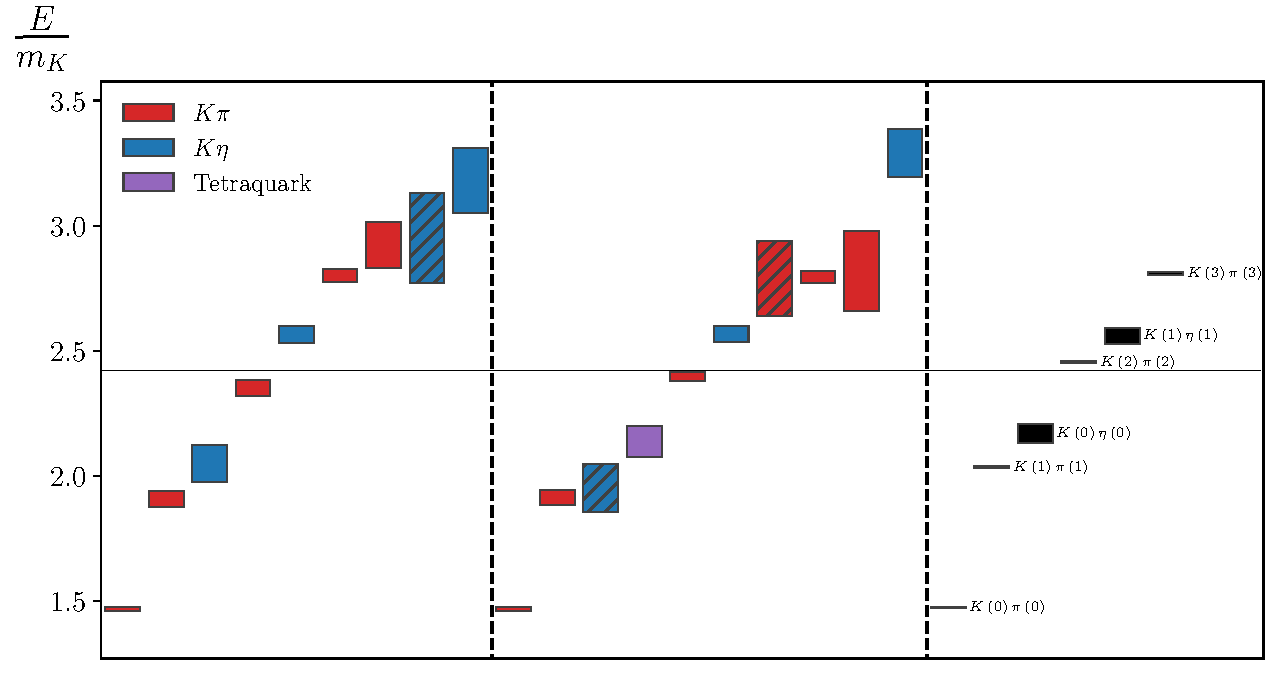
\includegraphics[width=\textwidth]{figures/spectrum_a1g/staircase.pdf}
  \caption{On the left: a spectrum obtained in the $\kappa$ channel using the operator basis given in Table~\ref{table:kappa_ops_no_tq}, which contains no tetraquark operators. In the middle: a spectrum obtained in the $\kappa$ channel using the same basis but with the addition of one tetraquark operator. On the right: two-particle non-interacting energies calculated from the rest-frame masses of the constituent particles, up to the point at which we have confidently saturated the basis with two-particle operators. The horizontal dash line indicates the four-particle $K\pi\pi\pi$ threshold. The color of a level indicates flavor content, determined by finding which operator has the largest overlap factor with that level. If the level has significant overlap with more than one operator (with the smaller overlap being $\geq 70\%$ of the larger overlap), then a hatched box is used to denote significant mixing.}
  \label{fig:kappa_spectrum}
\end{figure}

\begin{figure}
  \centering
  \hspace*{-0.5in}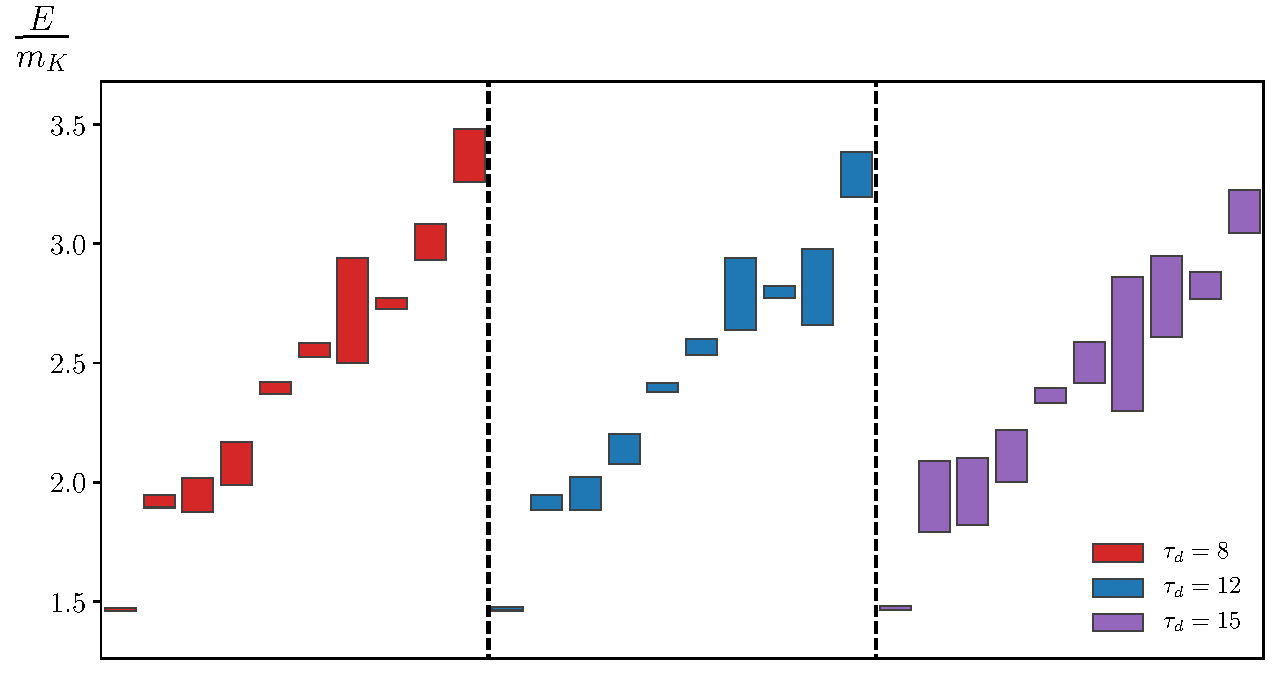
\includegraphics[width=\textwidth]{figures/spectrum_a1g/staircase_tau_d.pdf}
  \caption{The spectrum obtained using three different diagonalization times.}
  \label{fig:spectrum_td}
\end{figure}

\begin{figure}
  \raisebox{-0.05in}{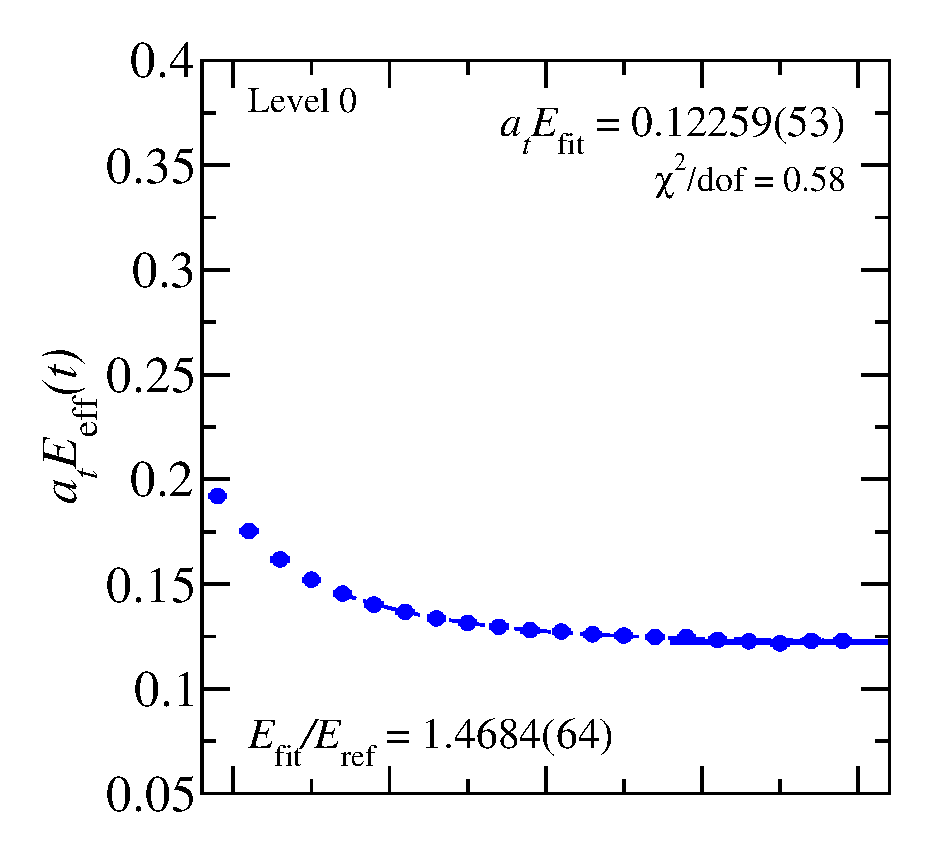
\includegraphics[width=0.34\textwidth]{figures/spectrum_a1g/no_tq/fits/fit_0.pdf}}
  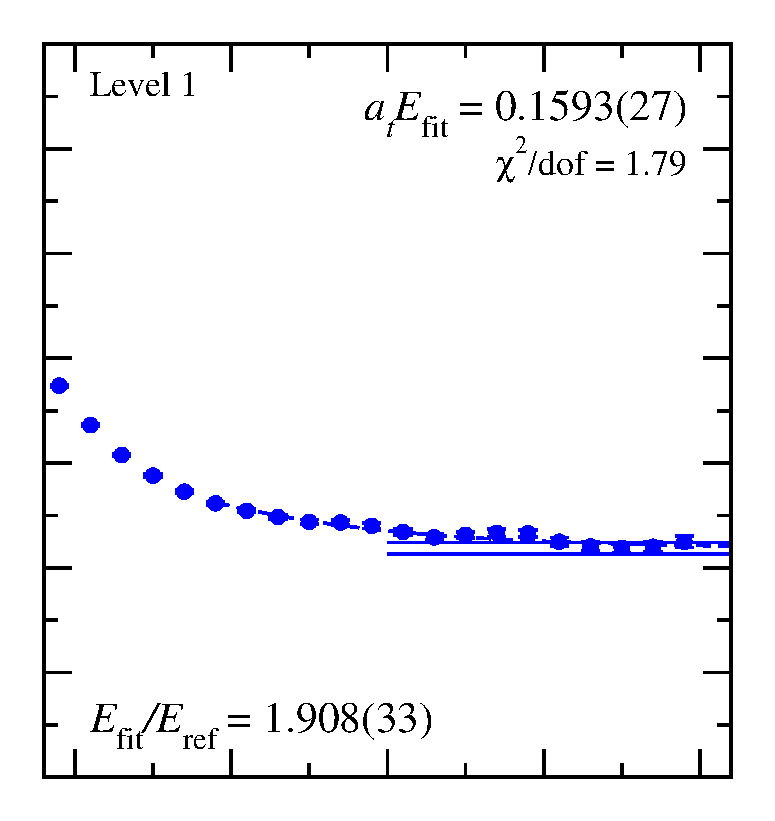
\includegraphics[width=0.28\textwidth]{figures/spectrum_a1g/no_tq/fits/fit_1.pdf}
  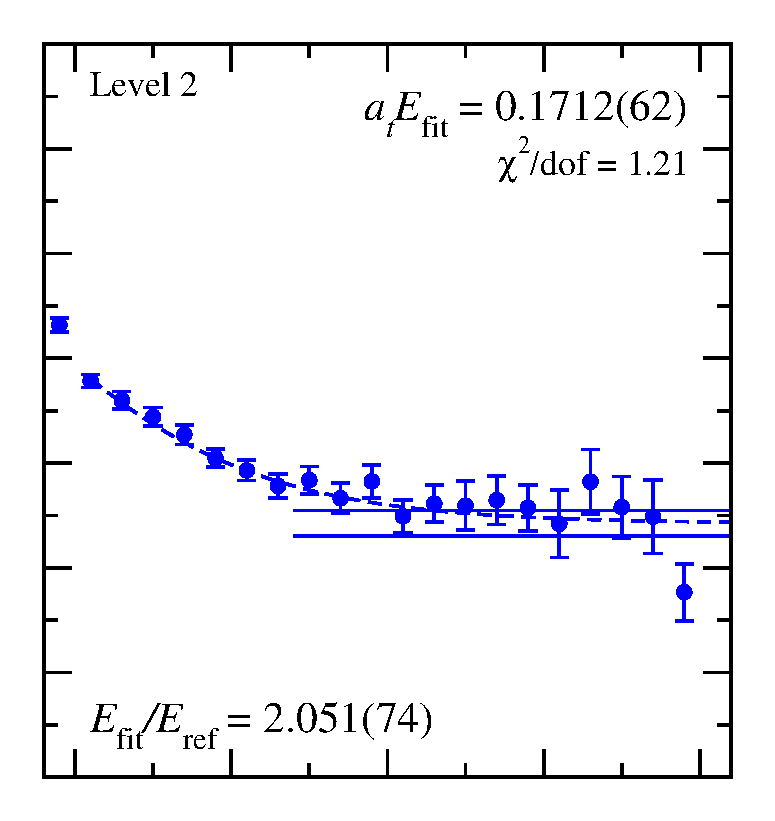
\includegraphics[width=0.28\textwidth]{figures/spectrum_a1g/no_tq/fits/fit_2.pdf}\\
  \raisebox{-0.05in}{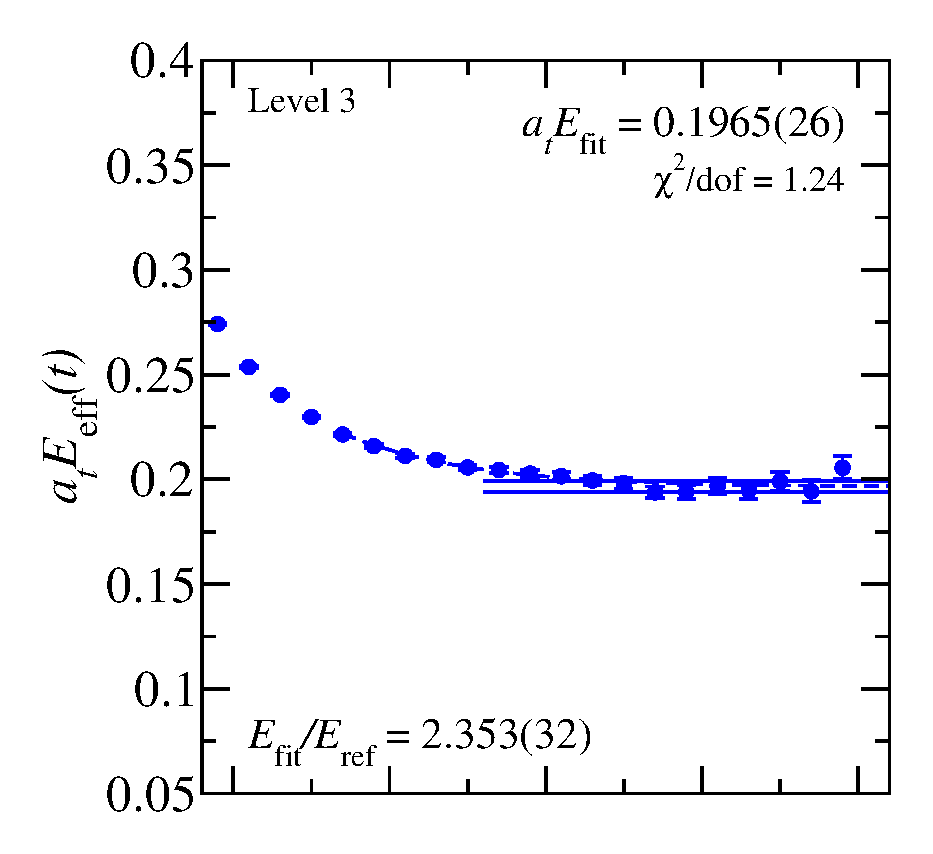
\includegraphics[width=0.34\textwidth]{figures/spectrum_a1g/no_tq/fits/fit_3.pdf}}
  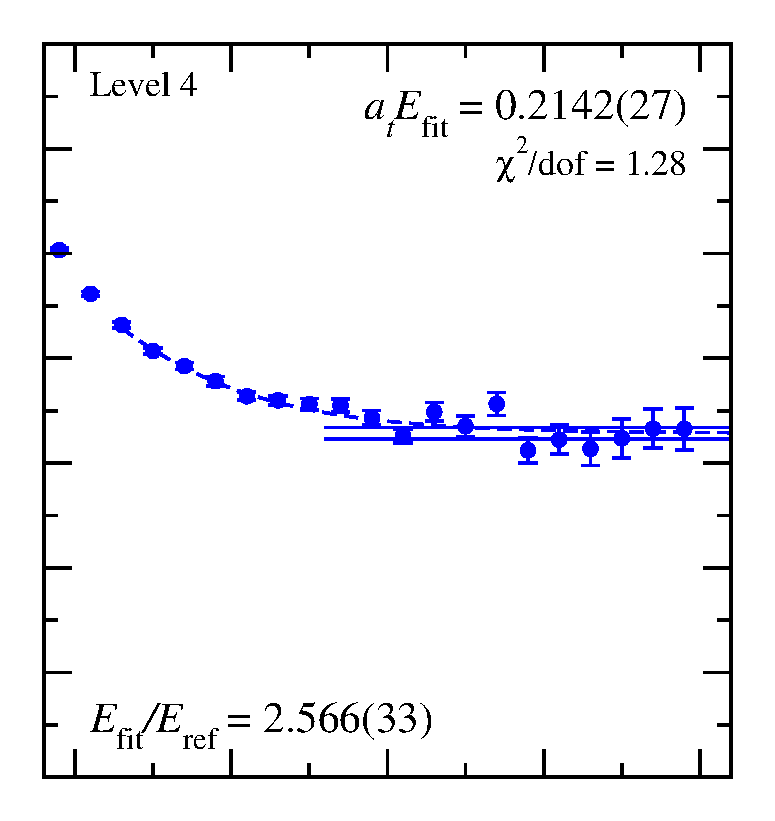
\includegraphics[width=0.28\textwidth]{figures/spectrum_a1g/no_tq/fits/fit_4.pdf}
  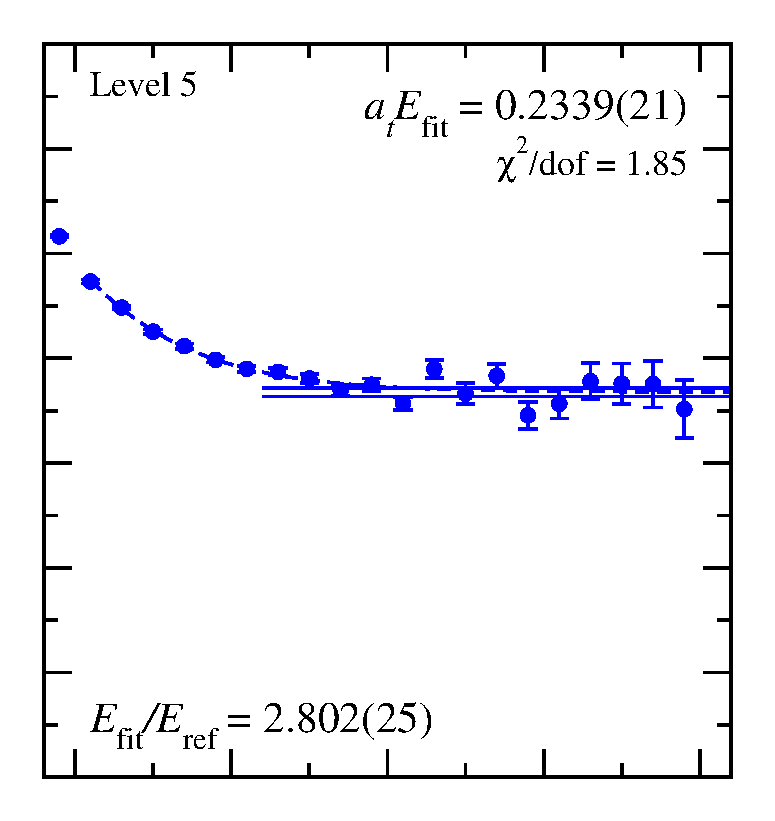
\includegraphics[width=0.28\textwidth]{figures/spectrum_a1g/no_tq/fits/fit_5.pdf}\\
  \raisebox{0.2in}{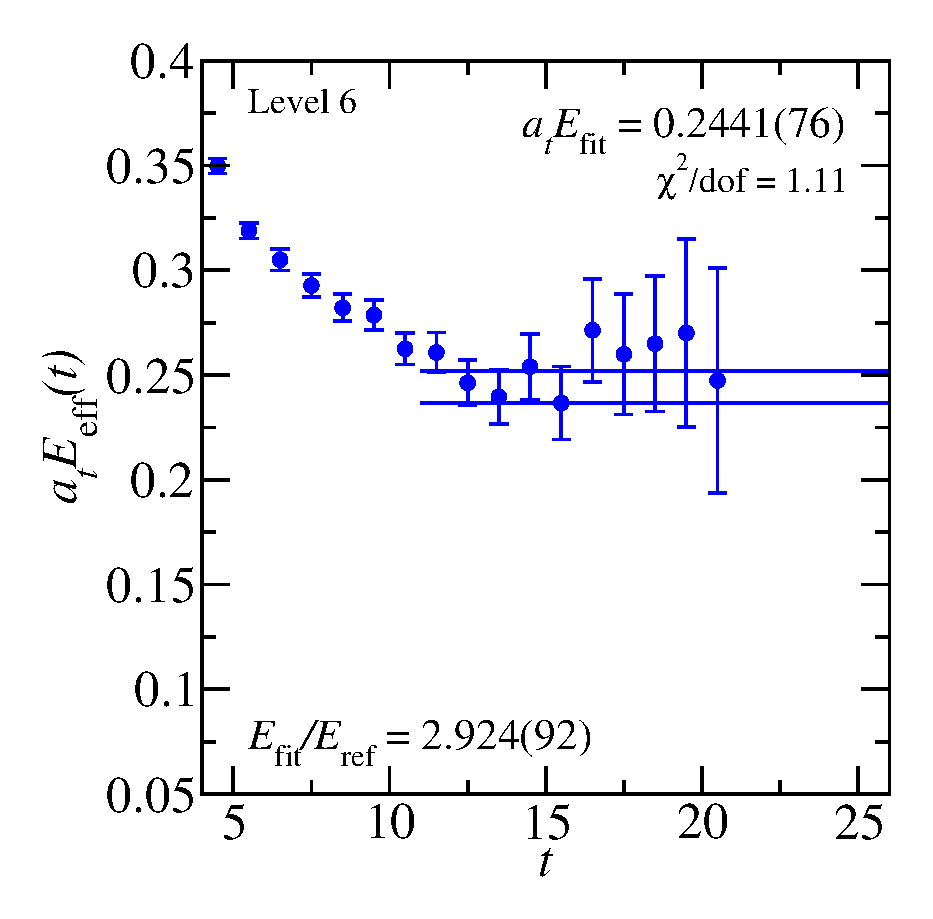
\includegraphics[width=0.34\textwidth]{figures/spectrum_a1g/no_tq/fits/fit_7.pdf}}
  \raisebox{0.2in}{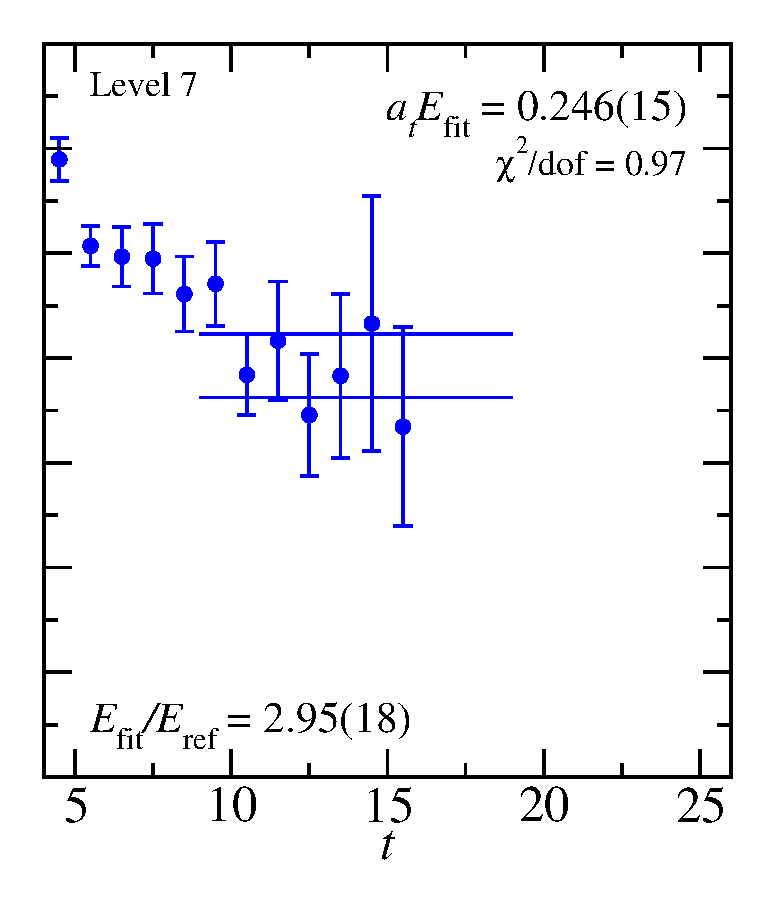
\includegraphics[width=0.28\textwidth]{figures/spectrum_a1g/no_tq/fits/fit_6.pdf}}
  \raisebox{0.2in}{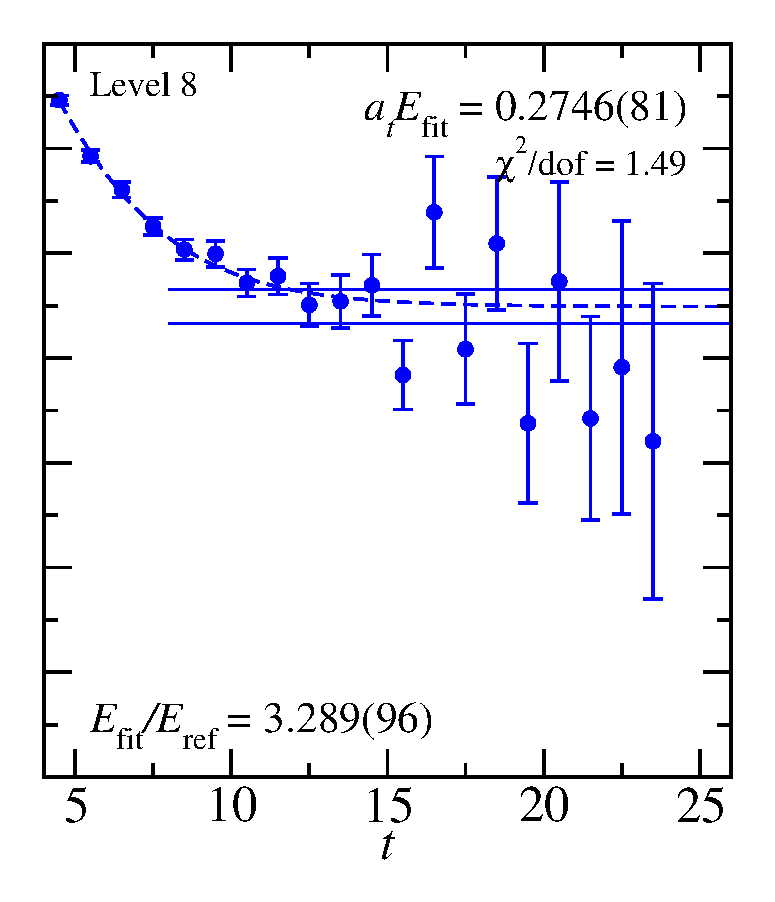
\includegraphics[width=0.28\textwidth]{figures/spectrum_a1g/no_tq/fits/fit_8.pdf}}
  \caption{Effective energies for the rotated $11\times 11$ correlator matrix in the $\kappa$ channel, using an operator basis containing no tetraquark operators. Effective energy curves calculated from correlator fits are overlaid, and fit results are shown.}
  \label{fig:kappa_no_tq_grid}
\end{figure}

\begin{figure}
  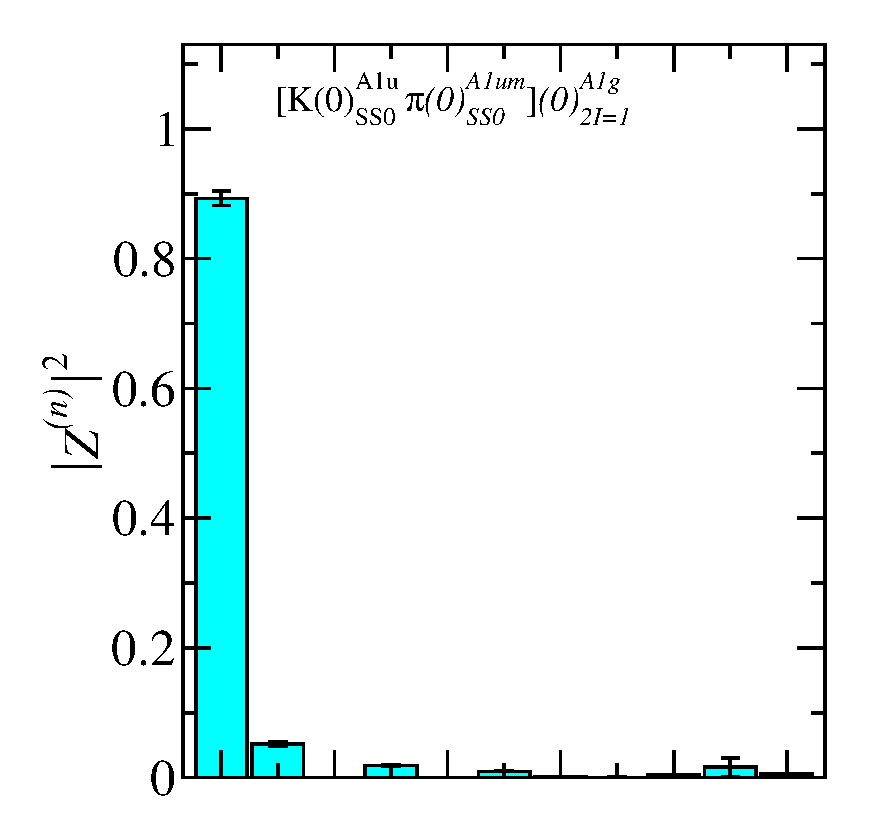
\includegraphics[width=0.3\textwidth]{figures/spectrum_a1g/no_tq/zfactors/zfactor_isodoublet_kaon_pion-A1g_1-P000-A1u-SS_0-P000-A1um-SS_0.pdf}
  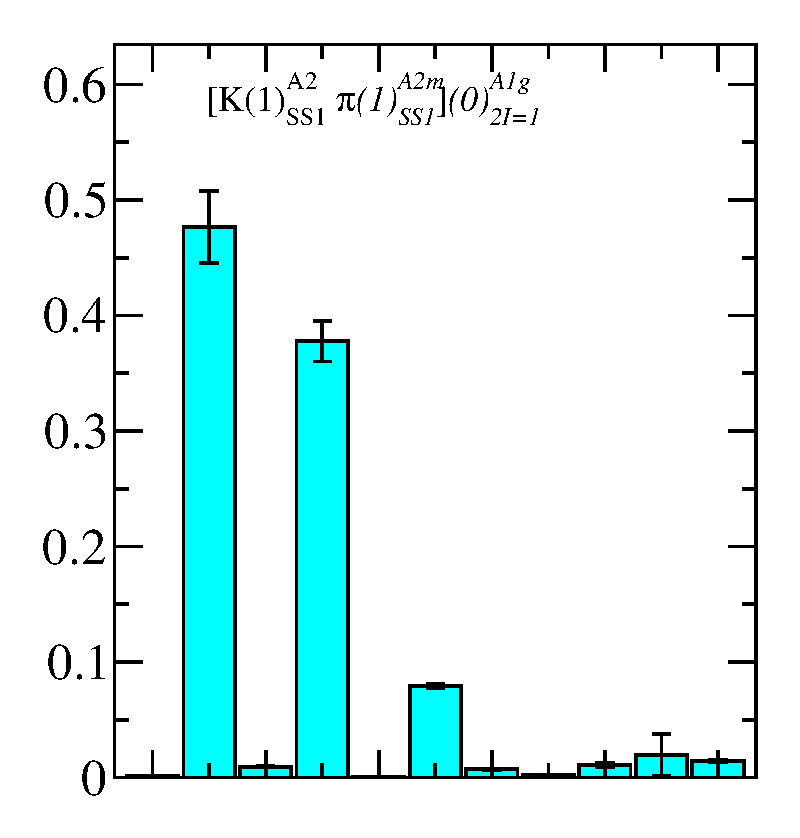
\includegraphics[width=0.28\textwidth]{figures/spectrum_a1g/no_tq/zfactors/zfactor_isodoublet_kaon_pion-A1g_1-P001-A2-SS_1-P00-1-A2m-SS_1.pdf}
  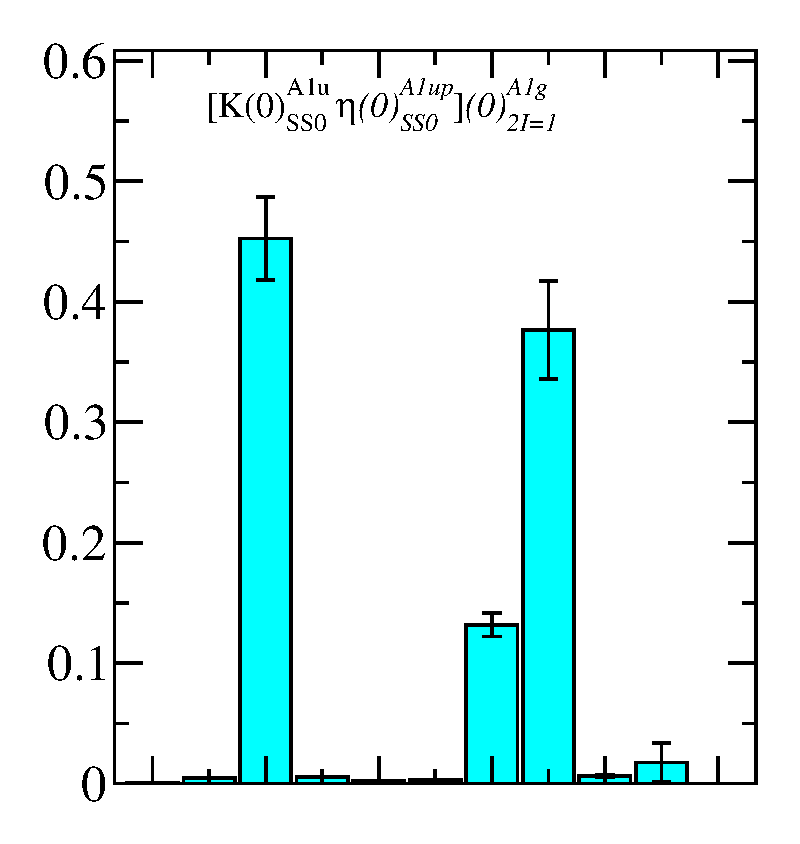
\includegraphics[width=0.28\textwidth]{figures/spectrum_a1g/no_tq/zfactors/zfactor_isodoublet_kaon_eta-A1g_1-P000-A1u-SS_0-P000-A1up-SS_0.pdf}\\
  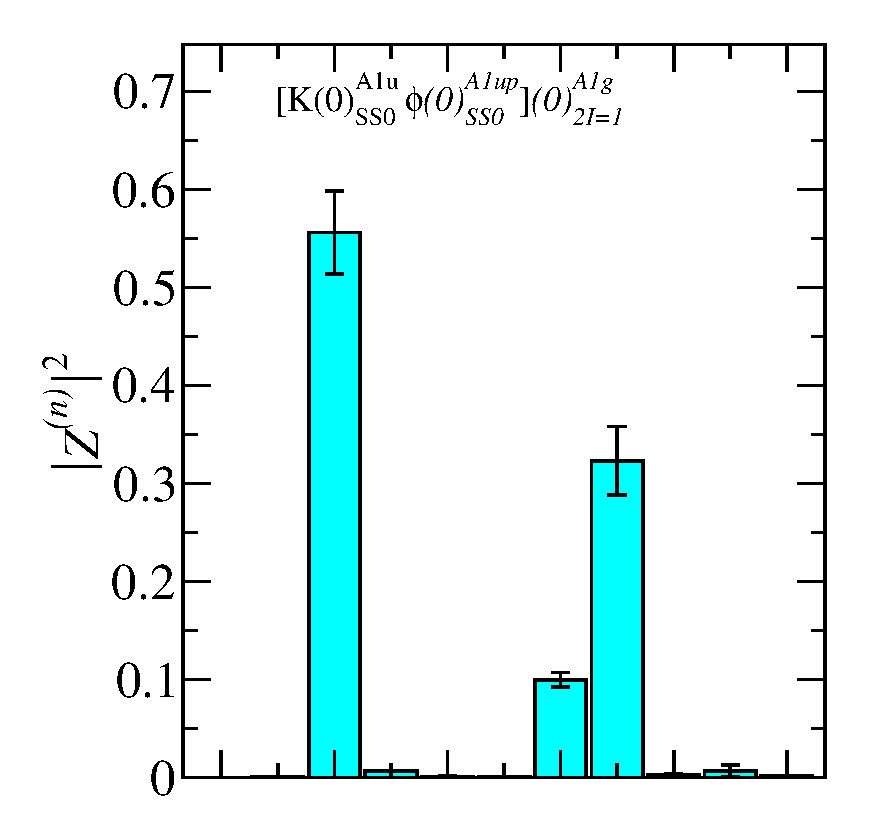
\includegraphics[width=0.3\textwidth]{figures/spectrum_a1g/no_tq/zfactors/zfactor_isodoublet_kaon_phi-A1g_1-P000-A1u-SS_0-P000-A1up-SS_0.pdf}
  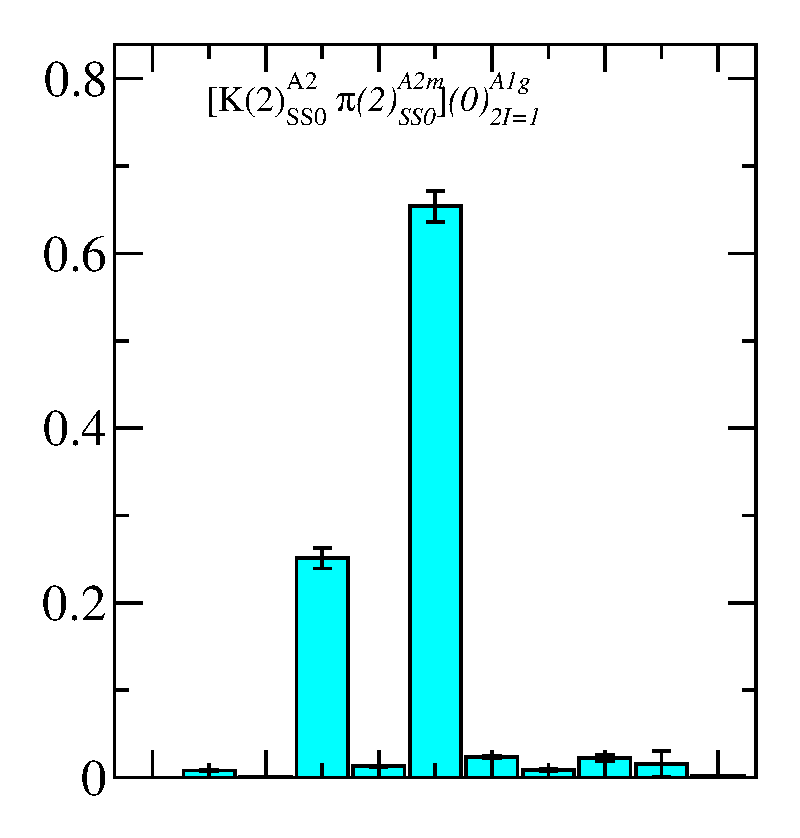
\includegraphics[width=0.28\textwidth]{figures/spectrum_a1g/no_tq/zfactors/zfactor_isodoublet_kaon_pion-A1g_1-P011-A2-SS_0-P0-1-1-A2m-SS_0.pdf}
  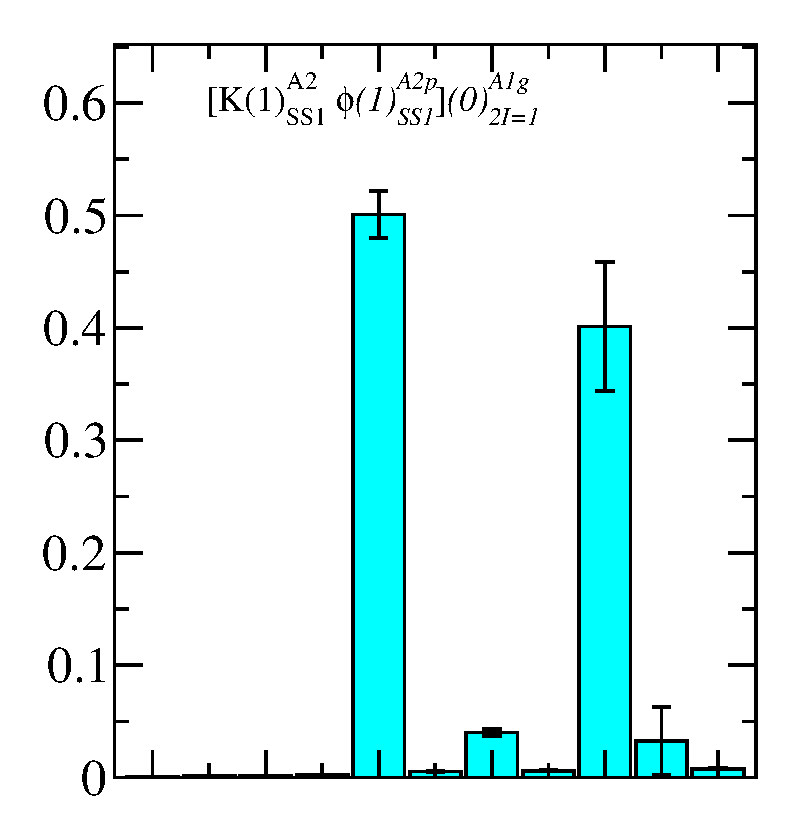
\includegraphics[width=0.28\textwidth]{figures/spectrum_a1g/no_tq/zfactors/zfactor_isodoublet_kaon_phi-A1g_1-P001-A2-SS_1-P00-1-A2p-SS_1.pdf}\\
  \raisebox{0.15in}{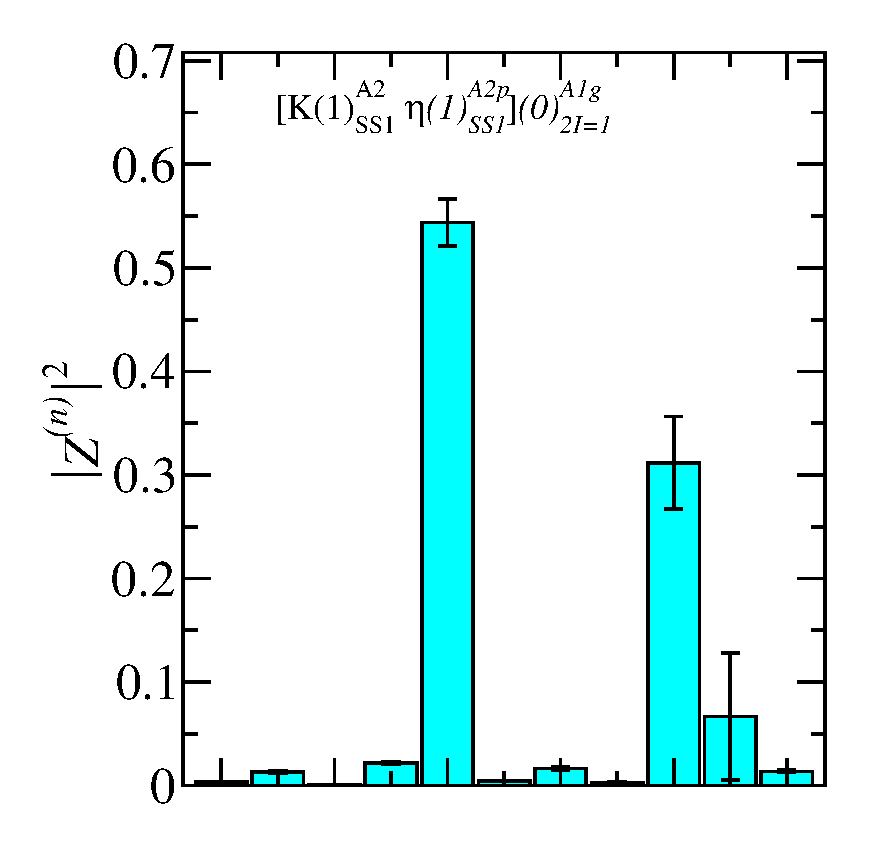
\includegraphics[width=0.3\textwidth]{figures/spectrum_a1g/no_tq/zfactors/zfactor_isodoublet_kaon_eta-A1g_1-P001-A2-SS_1-P00-1-A2p-SS_1.pdf}}
  \raisebox{0.15in}{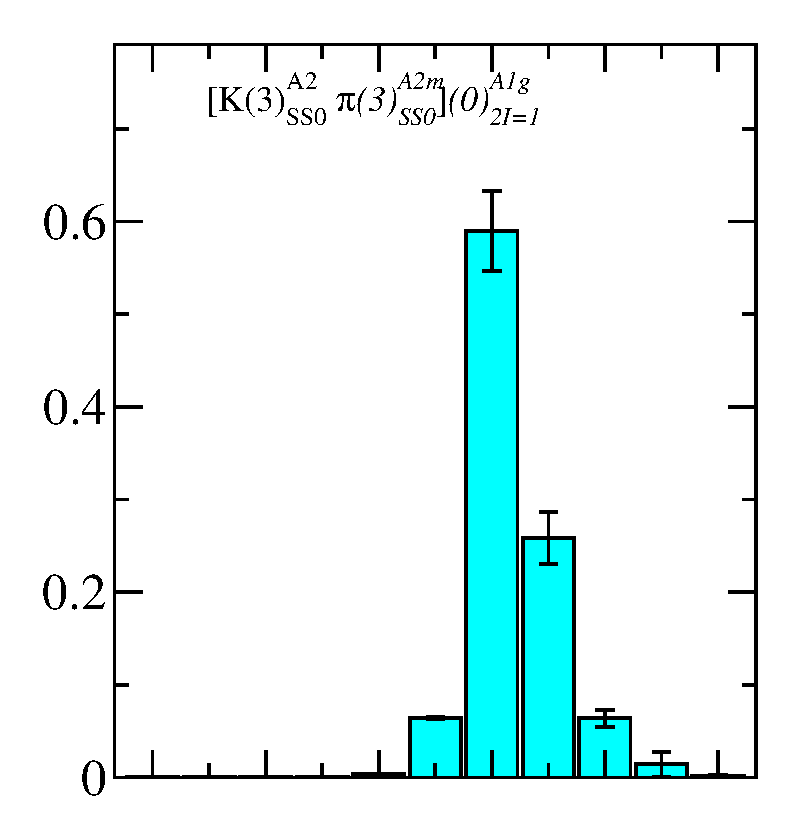
\includegraphics[width=0.28\textwidth]{figures/spectrum_a1g/no_tq/zfactors/zfactor_isodoublet_kaon_pion-A1g_1-P111-A2-SS_0-P-1-1-1-A2m-SS_0.pdf}}
  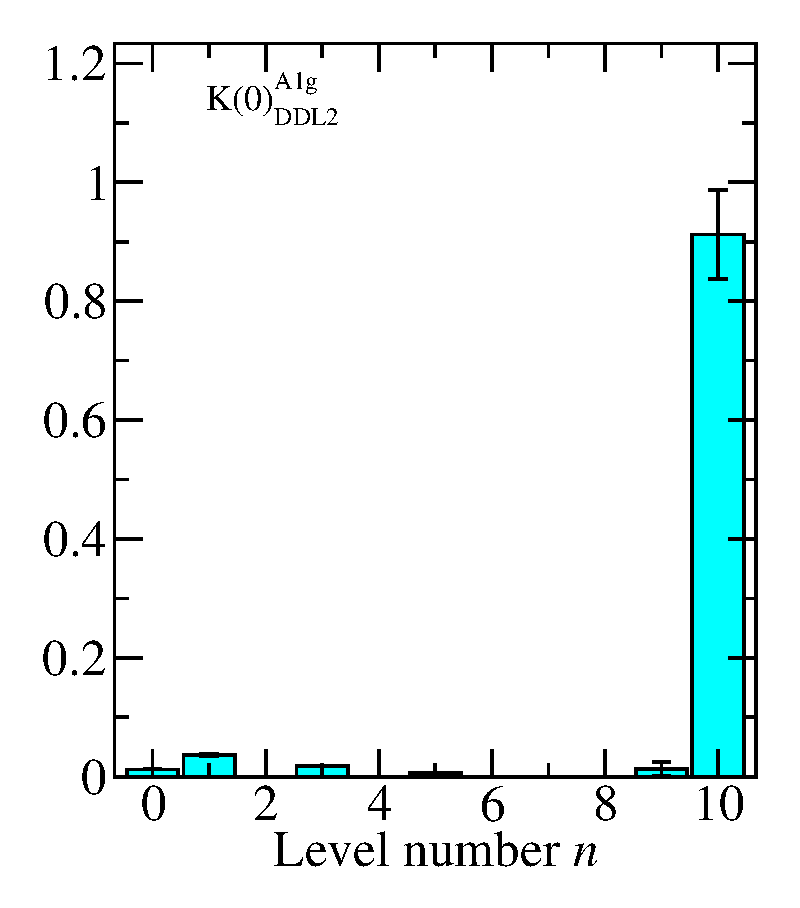
\includegraphics[width=0.28\textwidth]{figures/spectrum_a1g/no_tq/zfactors/zfactor_kaon-P000-A1g_1-DDL_2.pdf}\\
  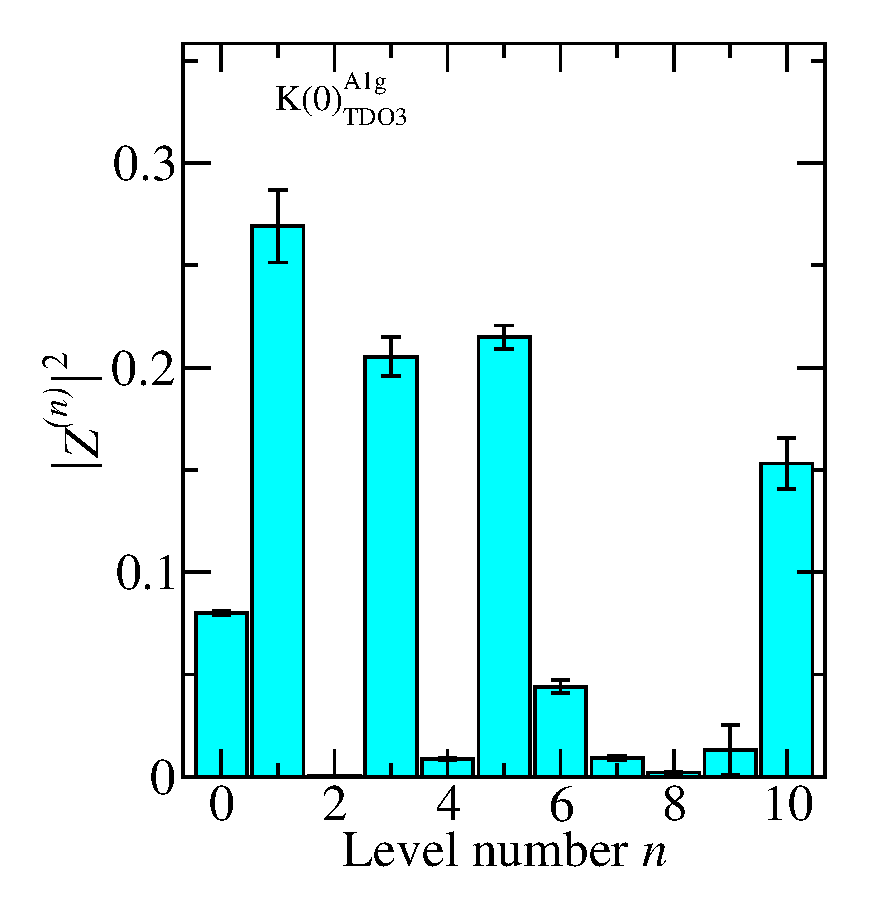
\includegraphics[width=0.3\textwidth]{figures/spectrum_a1g/no_tq/zfactors/zfactor_kaon-P000-A1g_1-TDO_3.pdf}
  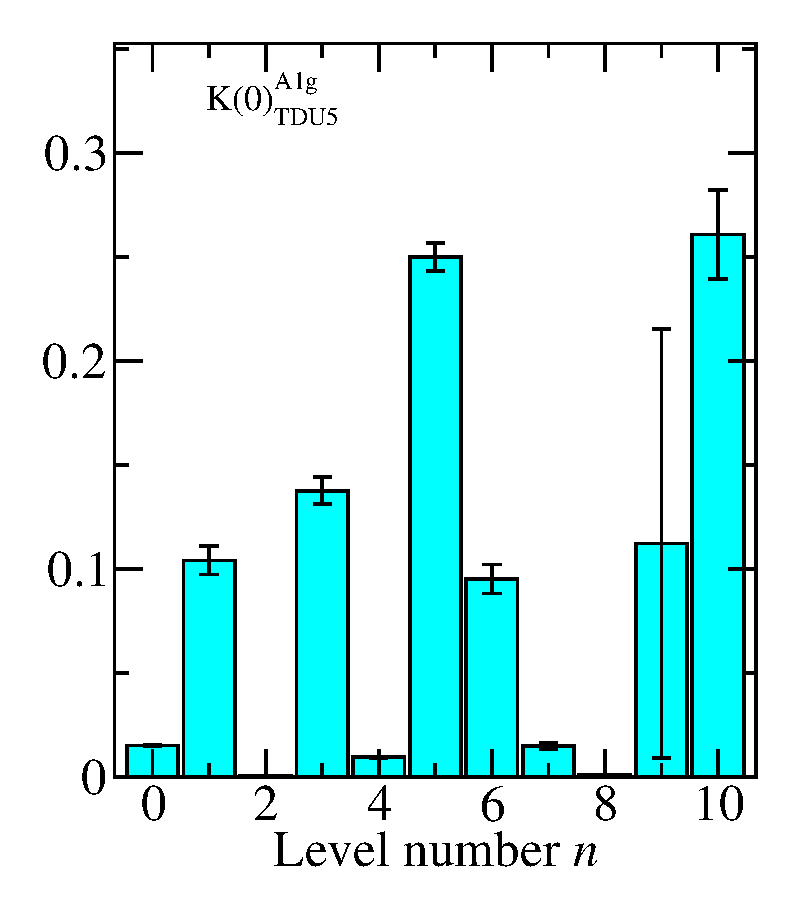
\includegraphics[width=0.28\textwidth]{figures/spectrum_a1g/no_tq/zfactors/zfactor_kaon-P000-A1g_1-TDU_5.pdf}
  \caption{Overlap factors for the rotated $11\times 11$ correlator matrix in the $\kappa$ channel, using an operator basis containing no tetraquark operators.}
  \label{fig:kappa_no_tq_zfactors}
\end{figure}

\begin{table}
  \centering
  \begin{tabular}{c|c|c|c|c}
    $E / E_K$ & $a_t E$ & Fit model & $(t_{\mathrm{min}}, {t_\mathrm{max}})$ & $\chi^2 / \rm{d.o.f.}$\\
    \hline
    1.4684(64)&0.12259(53)&2{-}exp&$(7, 26)$&0.58\\
1.908(33)&0.1593(27)&2{-}exp&$(8, 26)$&1.79\\%
2.051(74)&0.1712(62)&2{-}exp&$(4, 26)$&1.21\\
2.353(32)&0.1965(26)&2{-}exp&$(7, 26)$&1.24\\
2.566(33)&0.2142(27)&2{-}exp&$(5, 26)$&1.28\\
2.802(25)&0.2339(21)&2{-}exp&$(4, 26)$&1.85\\
2.924(92)&0.2441(76)&1{-}exp&$(11, 26)$&1.11\\
2.95(18)&0.246(15)&1{-}exp&$(9, 19)$&0.97\\
3.289(96)&0.2746(81)&2{-}exp&$(3, 26)$&1.49
  \end{tabular}
  \caption{Fit details for the spectrum obtained in the $\kappa$ channel using the operator basis given in Table~\ref{table:kappa_ops_no_tq}, which contains no tetraquark operators.}
  \label{table:kappa_no_tq_spectrum}
\end{table}

\begin{figure}
  \raisebox{-0.05in}{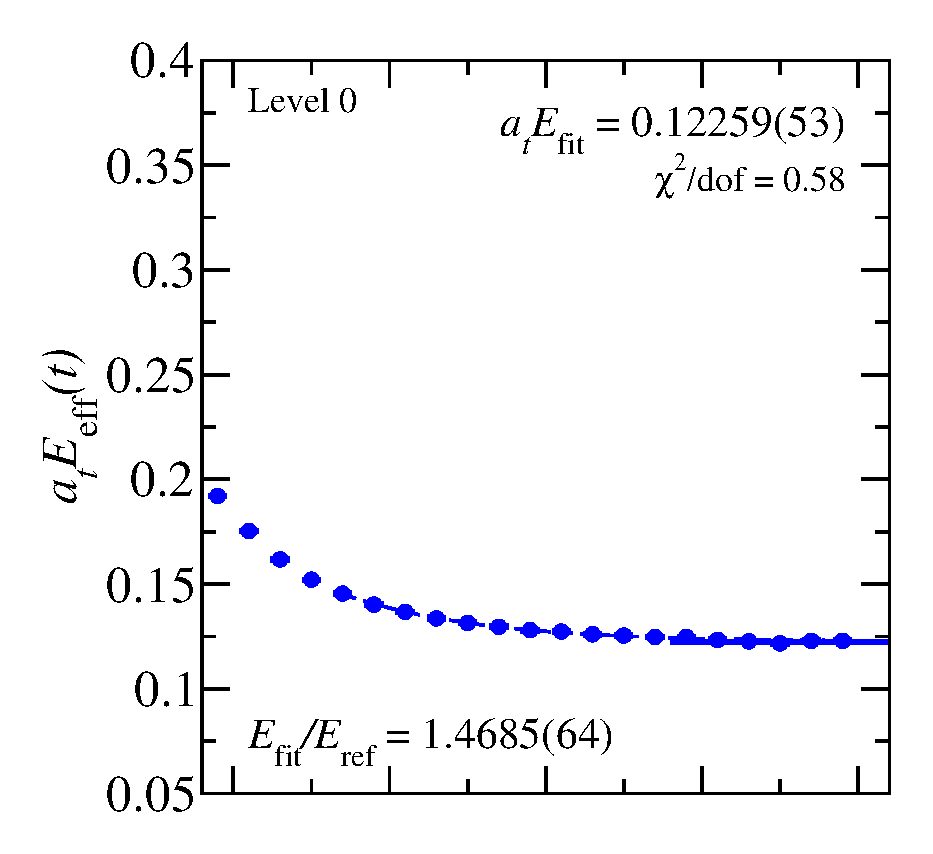
\includegraphics[width=0.34\textwidth]{figures/spectrum_a1g/with_tq/fits/fit_0.pdf}}
  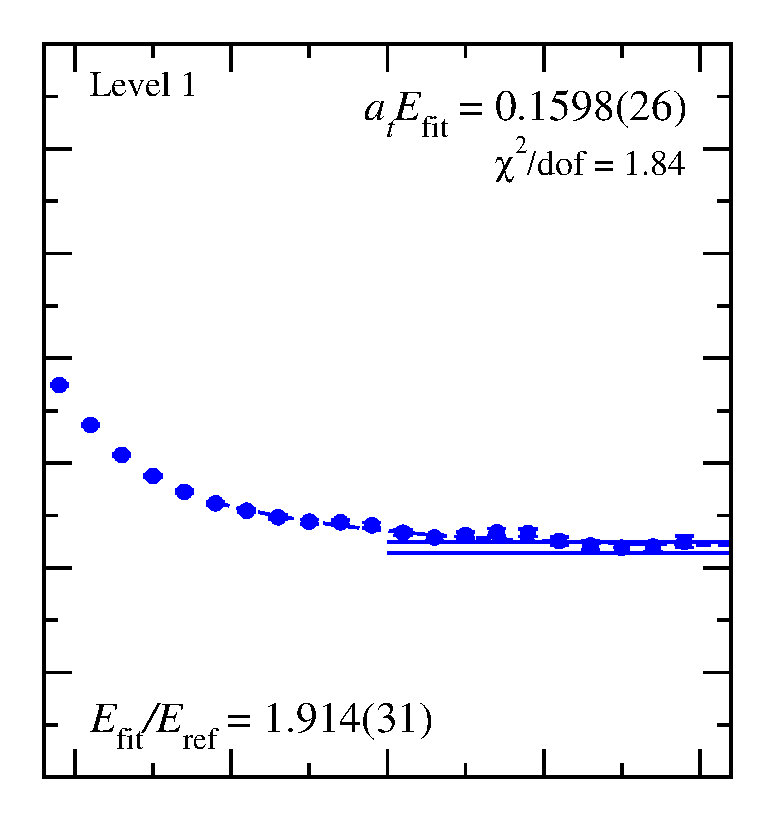
\includegraphics[width=0.28\textwidth]{figures/spectrum_a1g/with_tq/fits/fit_1.pdf}
  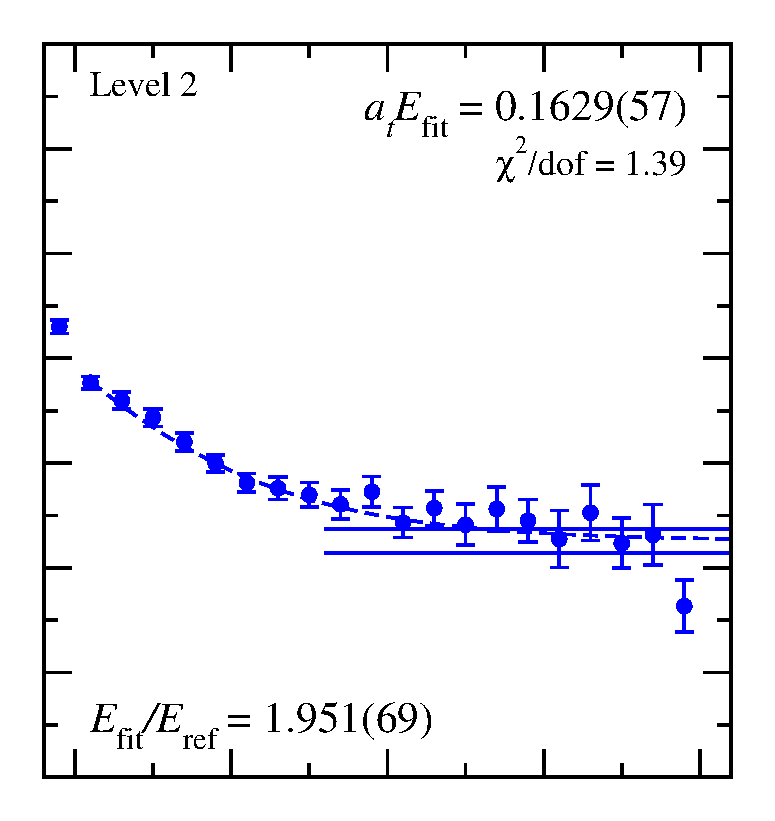
\includegraphics[width=0.28\textwidth]{figures/spectrum_a1g/with_tq/fits/fit_2.pdf}\\
  \raisebox{-0.05in}{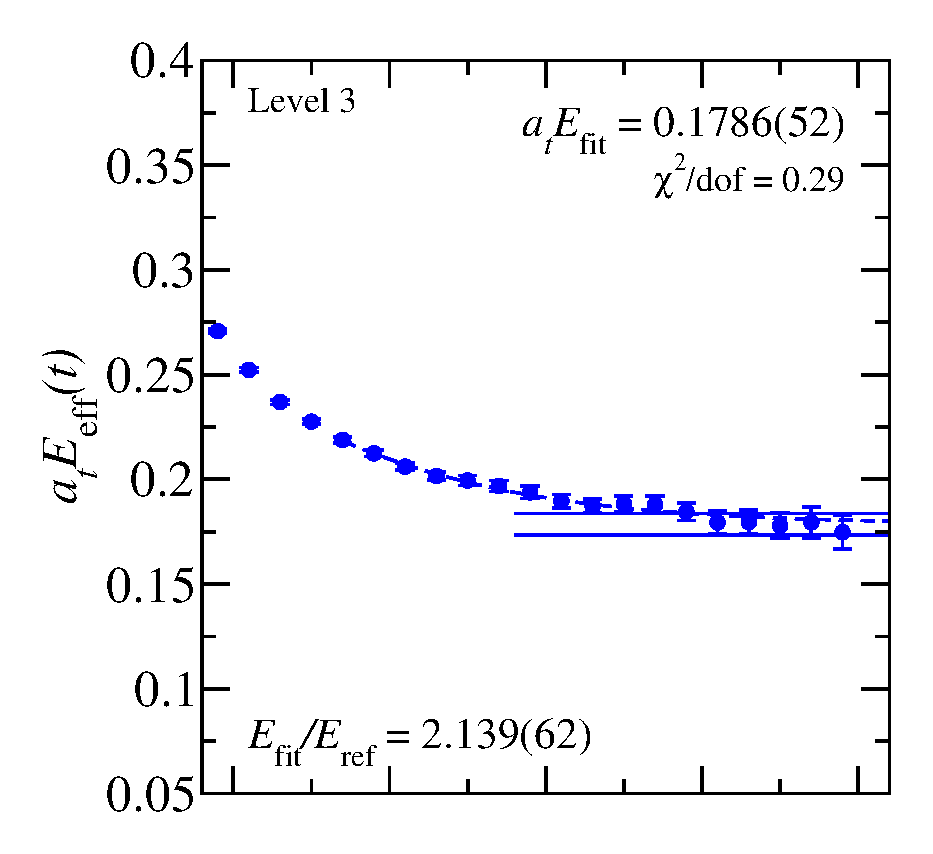
\includegraphics[width=0.34\textwidth]{figures/spectrum_a1g/with_tq/fits/fit_3.pdf}}
  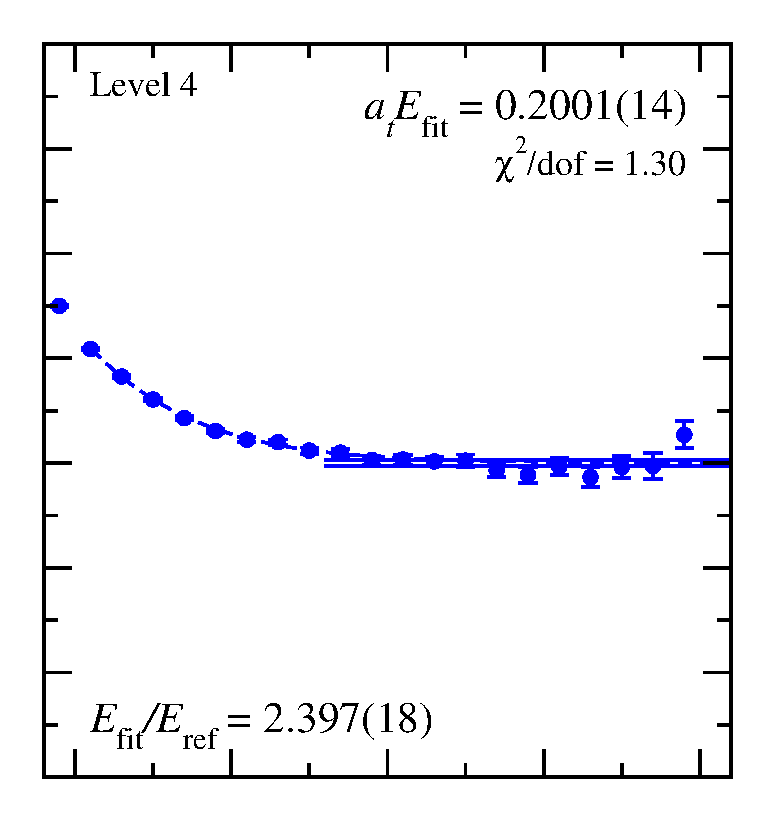
\includegraphics[width=0.28\textwidth]{figures/spectrum_a1g/with_tq/fits/fit_4.pdf}
  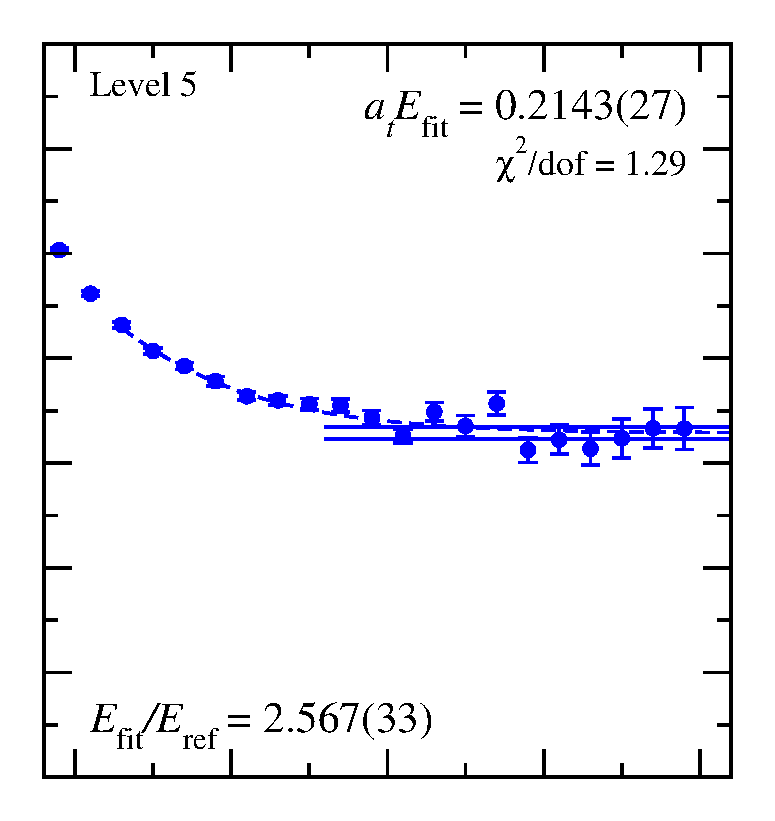
\includegraphics[width=0.28\textwidth]{figures/spectrum_a1g/with_tq/fits/fit_5.pdf}\\
  \raisebox{0.15in}{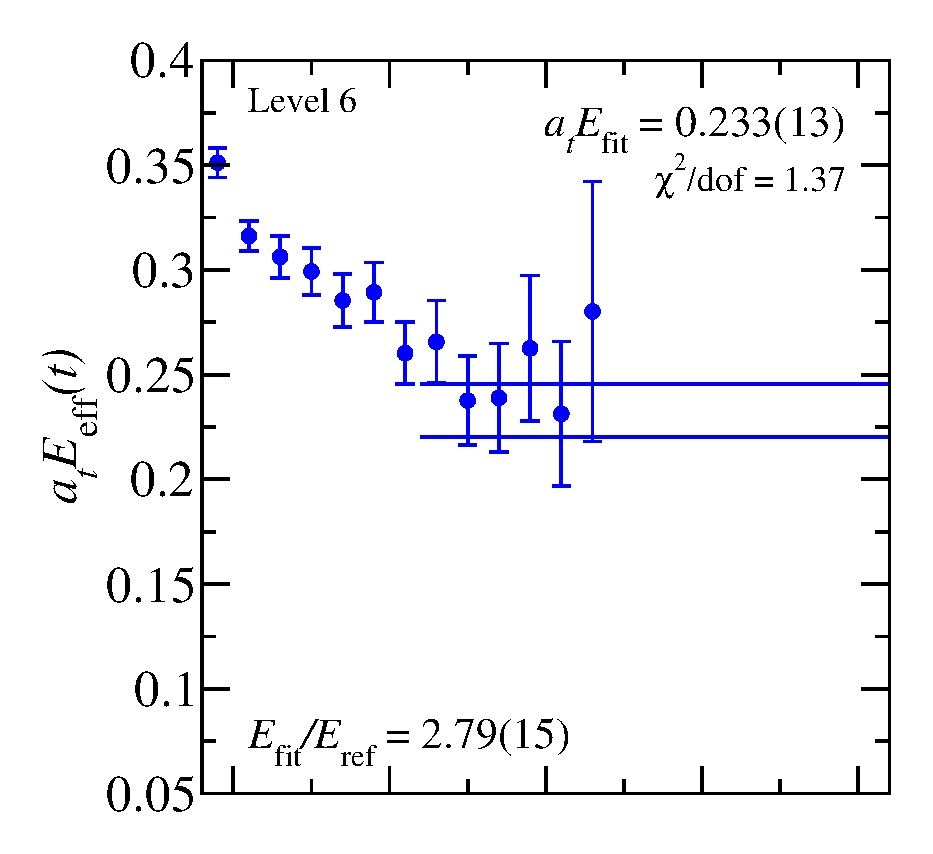
\includegraphics[width=0.34\textwidth]{figures/spectrum_a1g/with_tq/fits/fit_8.pdf}}
  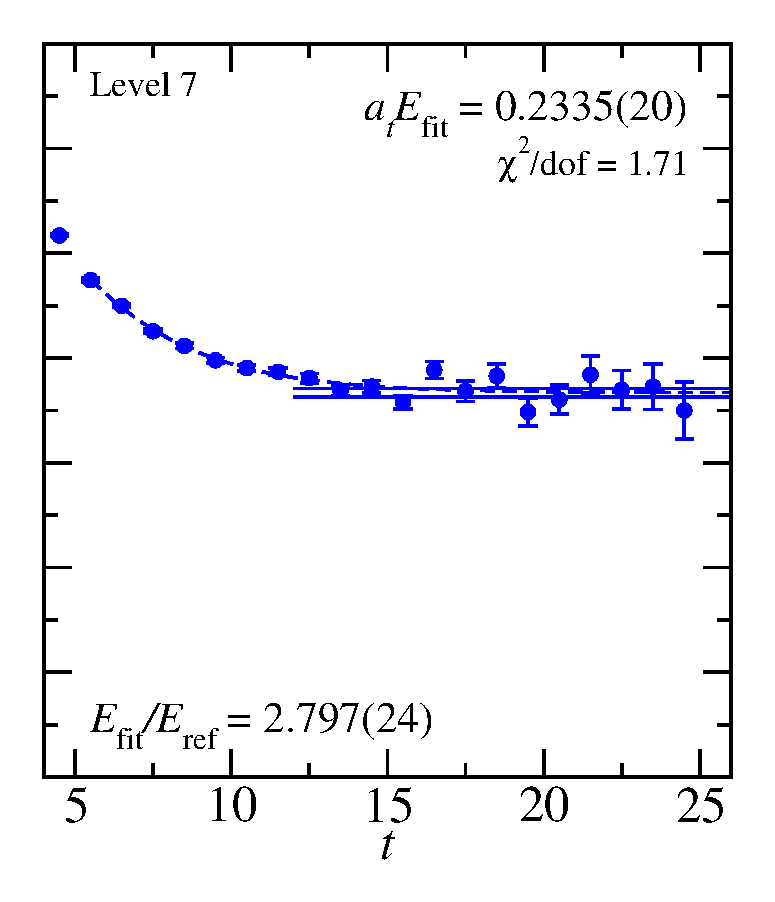
\includegraphics[width=0.28\textwidth]{figures/spectrum_a1g/with_tq/fits/fit_6.pdf}
  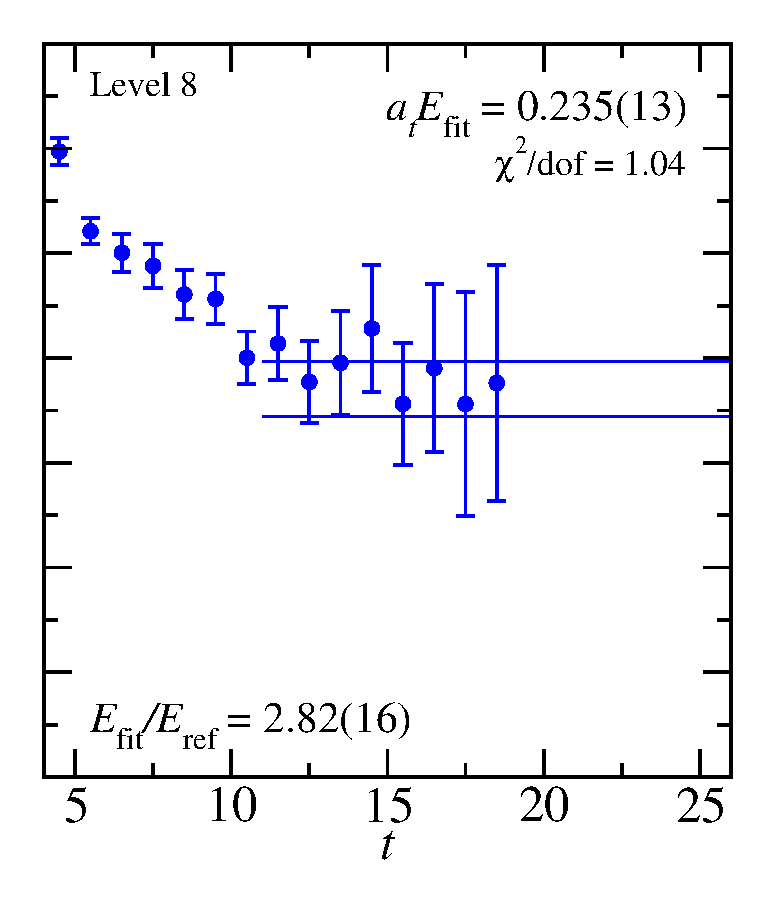
\includegraphics[width=0.28\textwidth]{figures/spectrum_a1g/with_tq/fits/fit_7.pdf}\\
  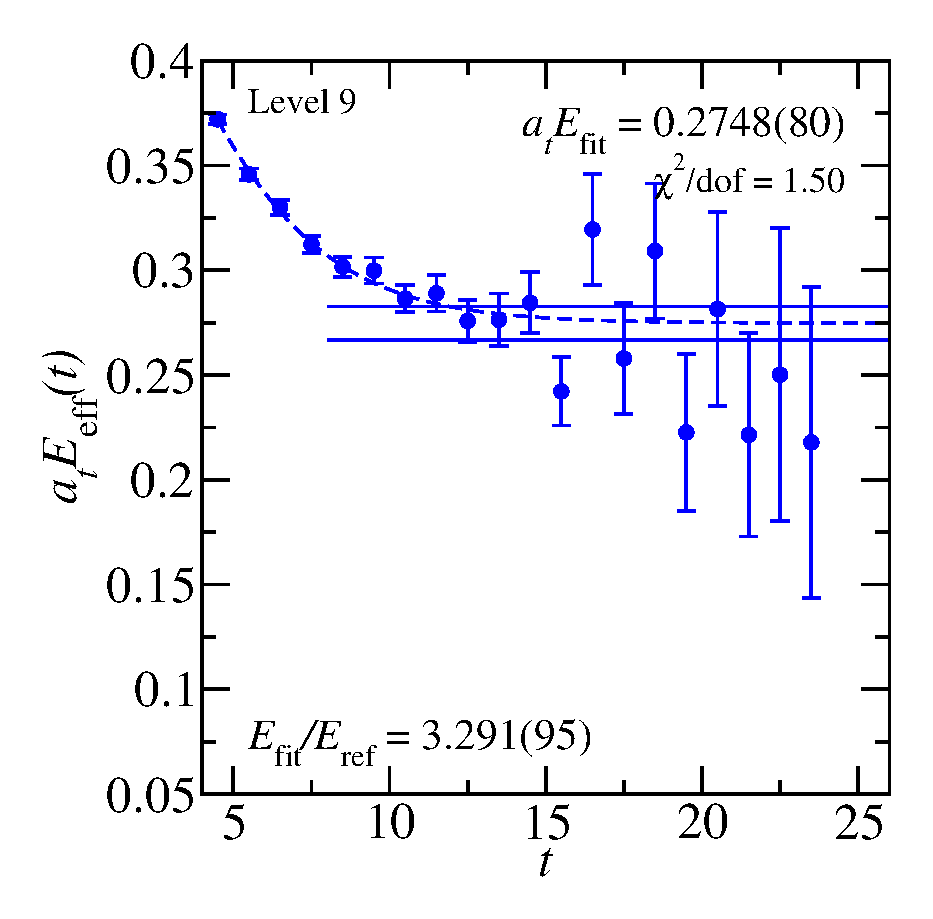
\includegraphics[width=0.34\textwidth]{figures/spectrum_a1g/with_tq/fits/fit_9.pdf}
  \caption{Effective energies for the rotated $12\times 12$ correlator matrix in the $\kappa$ channel, using the same operator basis but with the addition of one tetraquark operator. Effective energy curves calculated from correlator fits are overlaid, and fit results are shown.}
  \label{fig:kappa_with_tq_grid}
\end{figure}

\begin{figure}
  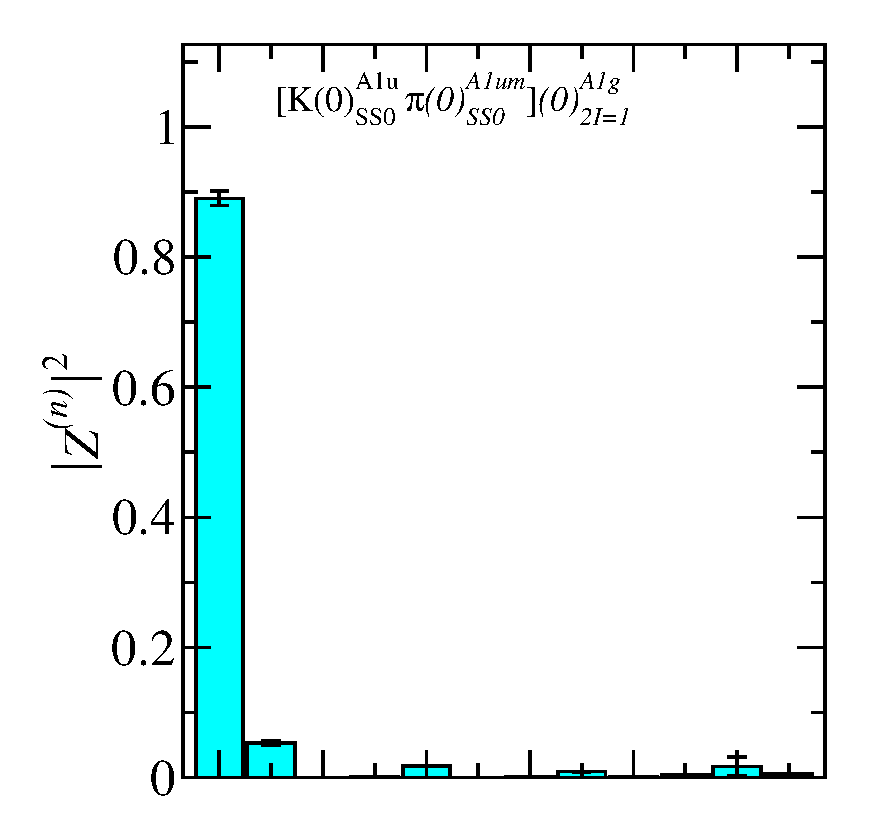
\includegraphics[width=0.3\textwidth]{figures/spectrum_a1g/with_tq/zfactors/zfactor_isodoublet_kaon_pion-A1g_1-P000-A1u-SS_0-P000-A1um-SS_0.pdf}
  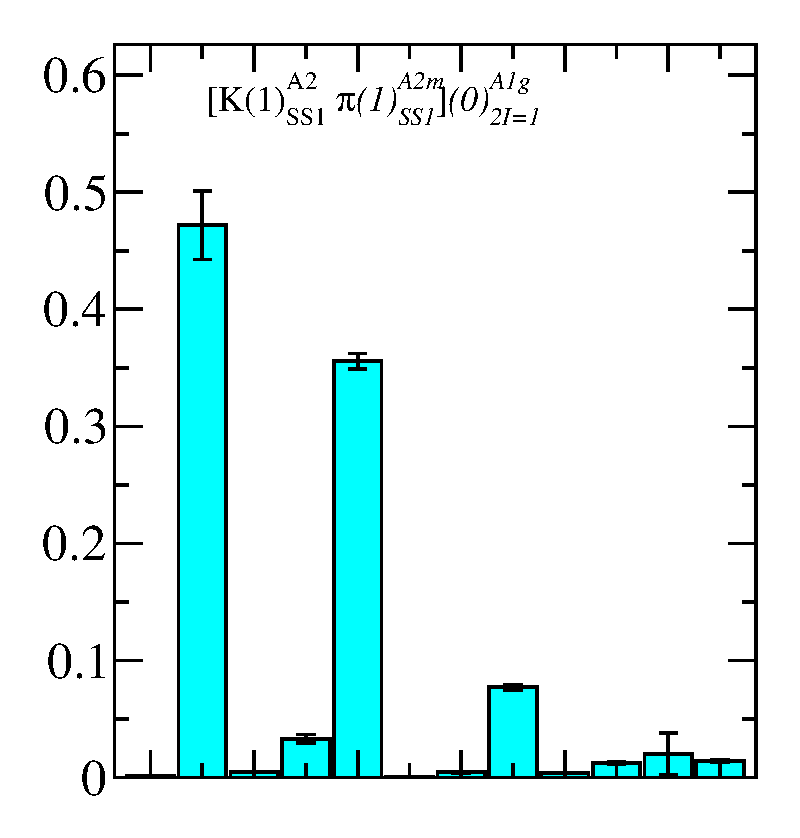
\includegraphics[width=0.28\textwidth]{figures/spectrum_a1g/with_tq/zfactors/zfactor_isodoublet_kaon_pion-A1g_1-P001-A2-SS_1-P00-1-A2m-SS_1.pdf}
  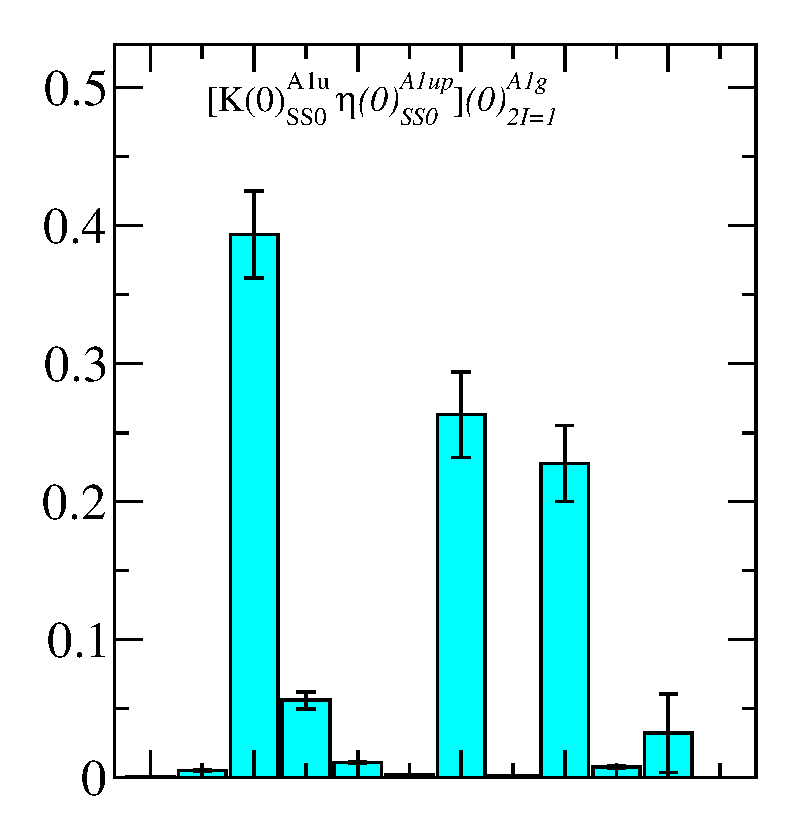
\includegraphics[width=0.28\textwidth]{figures/spectrum_a1g/with_tq/zfactors/zfactor_isodoublet_kaon_eta-A1g_1-P000-A1u-SS_0-P000-A1up-SS_0.pdf}\\
  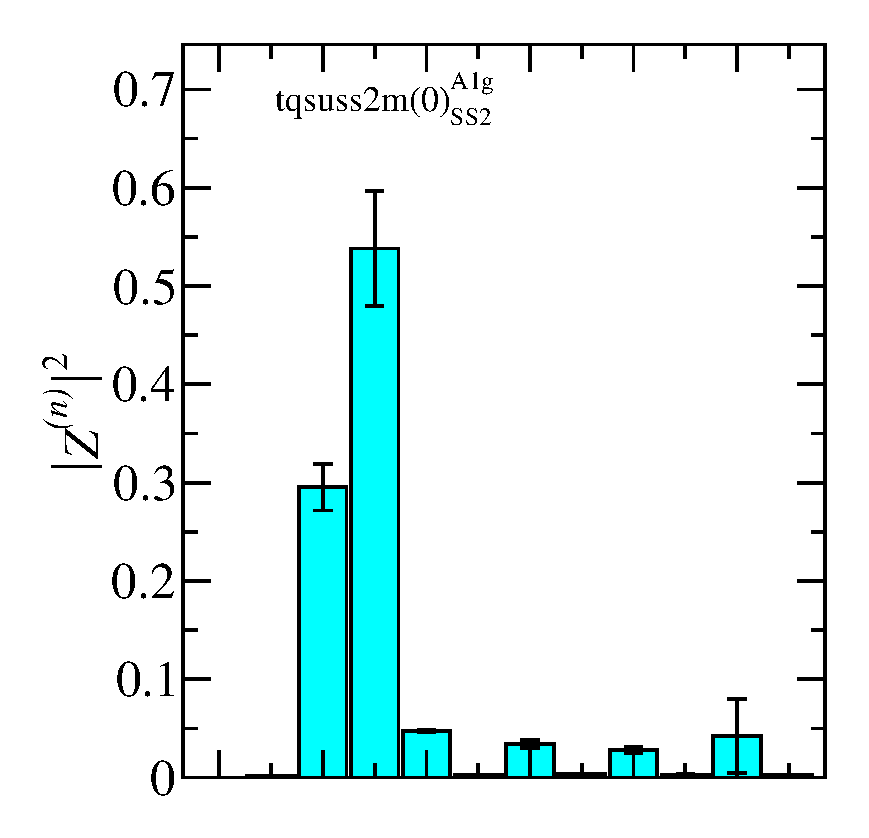
\includegraphics[width=0.3\textwidth]{figures/spectrum_a1g/with_tq/zfactors/zfactor_tqsuss2m-P000-A1g_1-SS_2.pdf}
  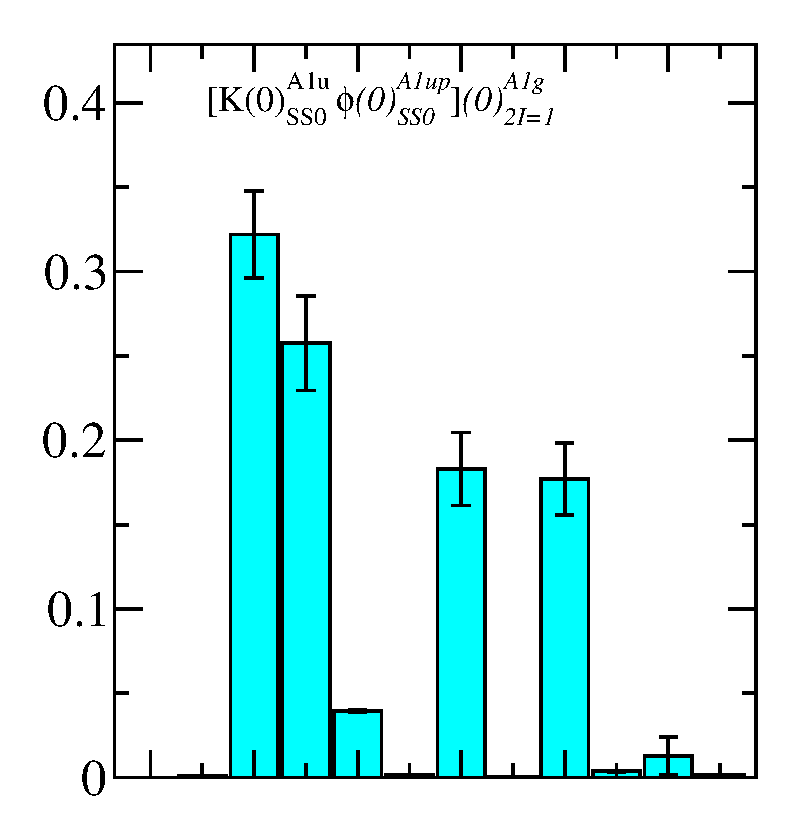
\includegraphics[width=0.28\textwidth]{figures/spectrum_a1g/with_tq/zfactors/zfactor_isodoublet_kaon_phi-A1g_1-P000-A1u-SS_0-P000-A1up-SS_0.pdf}
  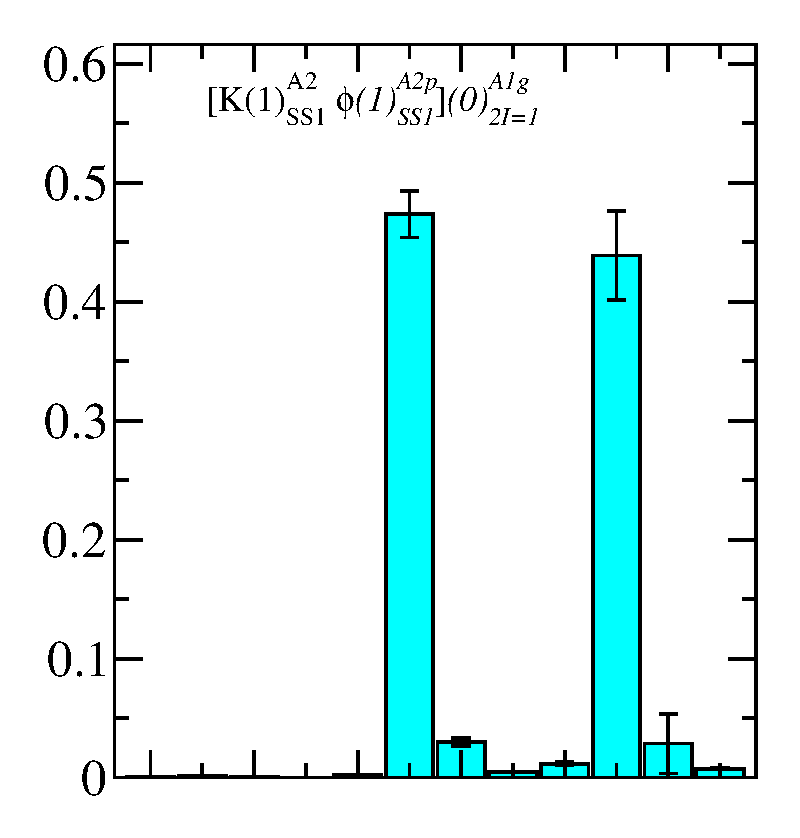
\includegraphics[width=0.28\textwidth]{figures/spectrum_a1g/with_tq/zfactors/zfactor_isodoublet_kaon_phi-A1g_1-P001-A2-SS_1-P00-1-A2p-SS_1.pdf}\\
  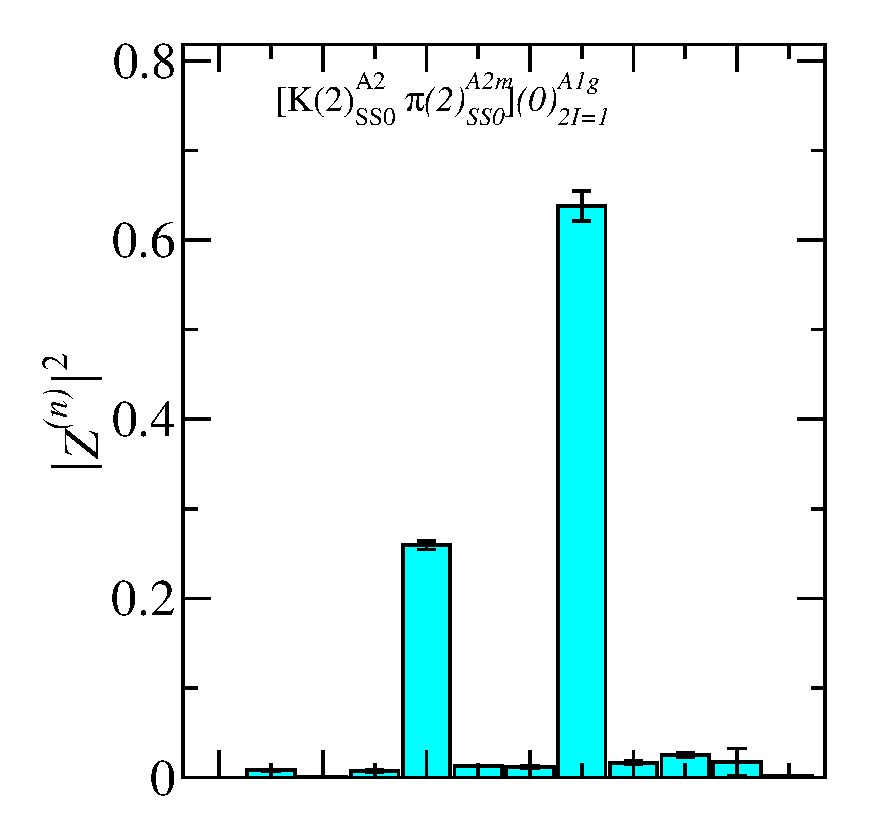
\includegraphics[width=0.3\textwidth]{figures/spectrum_a1g/with_tq/zfactors/zfactor_isodoublet_kaon_pion-A1g_1-P011-A2-SS_0-P0-1-1-A2m-SS_0.pdf}
  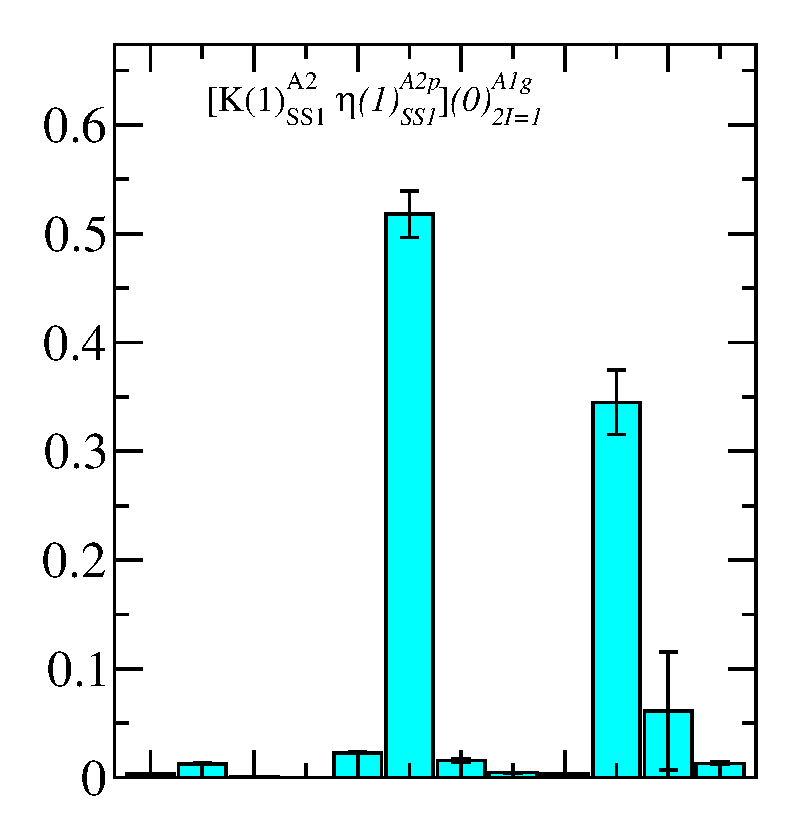
\includegraphics[width=0.28\textwidth]{figures/spectrum_a1g/with_tq/zfactors/zfactor_isodoublet_kaon_eta-A1g_1-P001-A2-SS_1-P00-1-A2p-SS_1.pdf}
  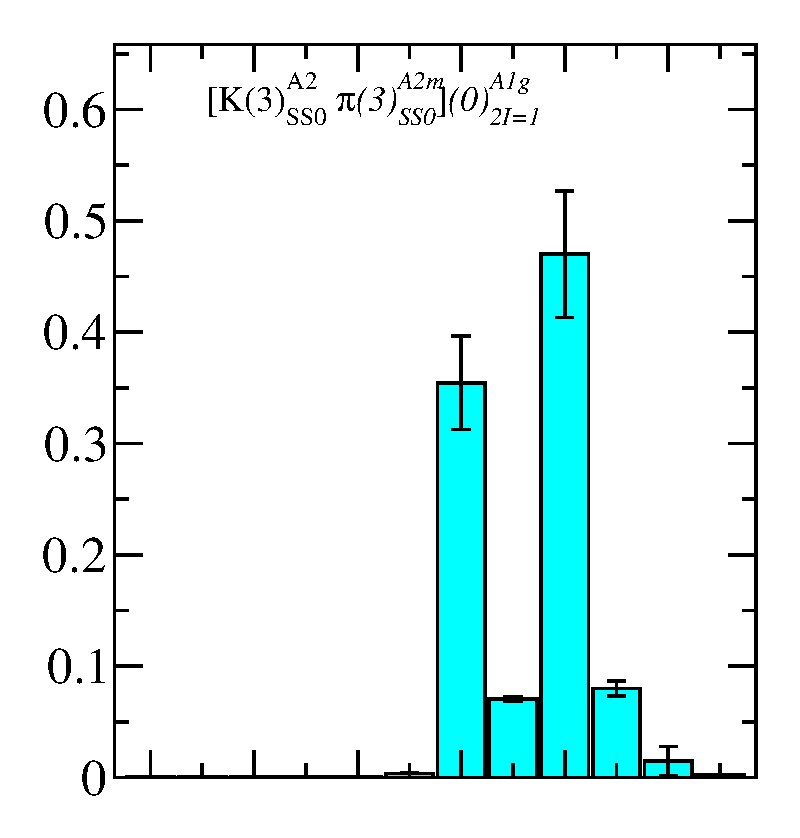
\includegraphics[width=0.28\textwidth]{figures/spectrum_a1g/with_tq/zfactors/zfactor_isodoublet_kaon_pion-A1g_1-P111-A2-SS_0-P-1-1-1-A2m-SS_0.pdf}\\
  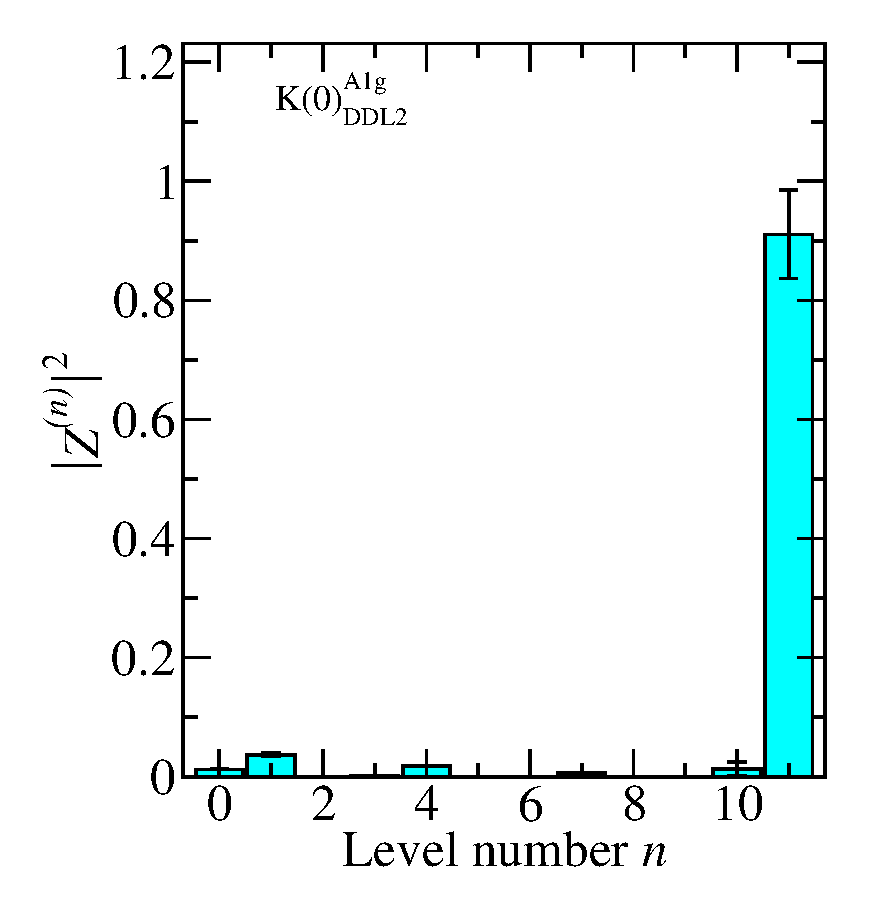
\includegraphics[width=0.3\textwidth]{figures/spectrum_a1g/with_tq/zfactors/zfactor_kaon-P000-A1g_1-DDL_2.pdf}
  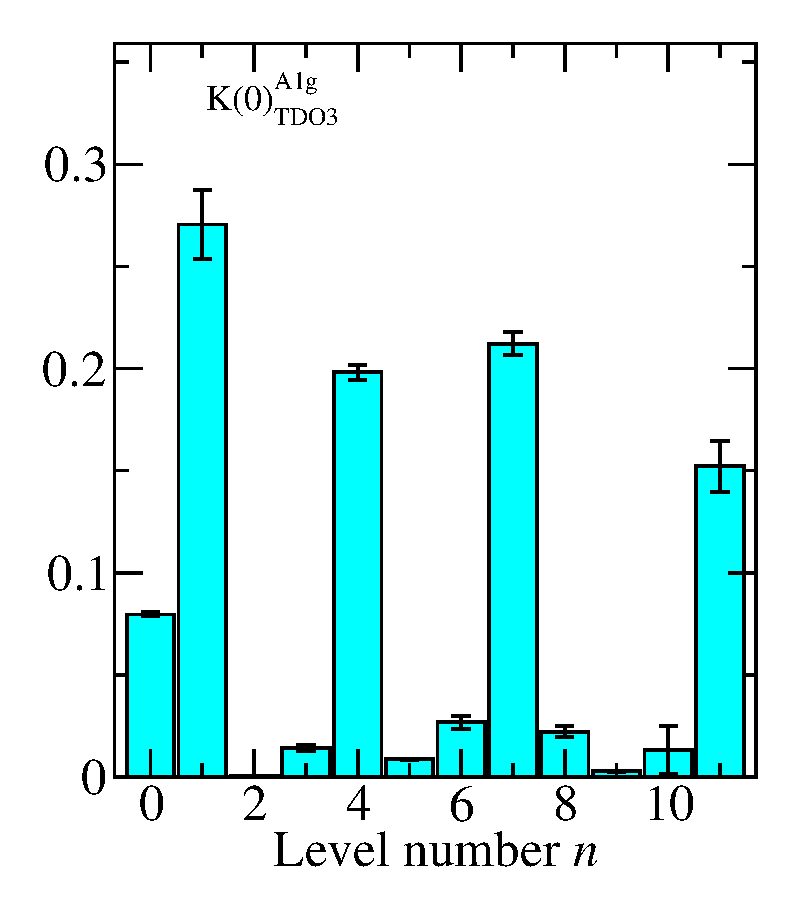
\includegraphics[width=0.28\textwidth]{figures/spectrum_a1g/with_tq/zfactors/zfactor_kaon-P000-A1g_1-TDO_3.pdf}
  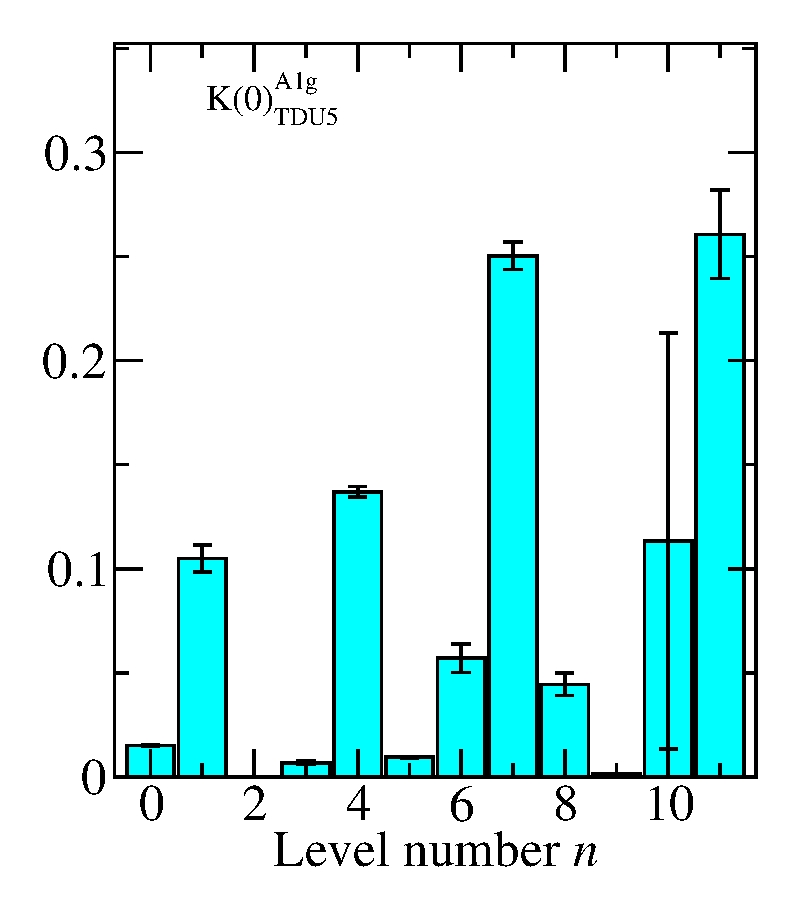
\includegraphics[width=0.28\textwidth]{figures/spectrum_a1g/with_tq/zfactors/zfactor_kaon-P000-A1g_1-TDU_5.pdf}
  \caption{Overlap factors for the rotated $12\times 12$ correlator matrix in the $\kappa$ channel, using the same operator basis but with the addition of one tetraquark operator.}
  \label{fig:kappa_with_tq_zfactors}
\end{figure}

\begin{table}
  \centering
  \begin{tabular}{c|c|c|c|c}
    $E / E_K$ & $a_t E$ & Fit model & $(t_{\mathrm{min}}, {t_\mathrm{max}})$ & $\chi^2 / \rm{d.o.f.}$\\
    \hline
    1.4685(64)&0.12259(53)&2{-}exp&$(7, 26)$&0.58\\
    1.914(31)&0.1598(26)&2{-}exp&$(8, 26)$&1.84\\
    1.951(69)&0.1629(57)&2{-}exp&$(4, 26)$&1.39\\
    2.139(62)&0.1786(52)&2{-}exp&$(7, 26)$&0.29\\
    2.397(18)&0.2001(14)&2{-}exp&$(4, 26)$&1.3\\
    2.567(33)&0.2143(27)&2{-}exp&$(5, 26)$&1.29\\
    2.79(15)&0.233(13)&1{-}exp&$(11, 26)$&1.37\\
    2.797(24)&0.2335(20)&2{-}exp&$(4, 26)$&1.71\\
    2.82(16)&0.235(13)&1{-}exp&$(11, 26)$&1.04\\
    3.291(95)&0.2748(80)&2{-}exp&$(3, 26)$&1.5
  \end{tabular}
  \caption{Fit details for the spectrum obtained in the $\kappa$ channel using the same operator basis but with the addition of one tetraquark operator.}
  \label{table:kappa_with_tq_spectrum}
\end{table}

\section{$a_0(980)$ Channel}
\subsection{Operator Bases}
\begin{table}
  \centering
  \begin{tabular}{l|l}
    \textbf{Single-Hadron Operators} & \textbf{Two-Hadron Operators}\\
    \hline
    $\pi^{\rm{SS}0}_{A_{1g}^-}$ & $K(0)^{\rm{SS}0}_{A_{1u}}\; \overline K(0)^{\rm{SS}0}_{A_{1u}}$\\
    $\pi^{\rm{TDO}3}_{A_{1g}^-}$ & $K(1)^{\rm{SS}1}_{A_{2}}\; \overline K(1)^{\rm{SS}1}_{A_{2}}$ \\
    $\pi^{\rm{SD}2}_{A_{1g}^-}$ & $\eta(0)^{\rm{SS}0}_{T_{1u}^-}\; \pi(0)^{\rm{SS}0}_{T_{1u}^+}$ \\
    & $\eta(1)^{\rm{SS}0}_{A_{2}^+}\; \pi(1)^{\rm{SS}0}_{A_{2}^-}$ \\
    & $\eta(2)^{\rm{SS}1}_{A_{2}^+}\; \pi(2)^{\rm{SS}1}_{A_{2}^-}$ \\
    & $\phi(0)^{\rm{SS}0}_{A_{1u}^+}\; \pi(0)^{\rm{SS}0}_{A_{1u}^-}$ \\
    & $\phi(0)^{\rm{SS}0}_{T_{1u}^-}\; \pi(0)^{\rm{SS}0}_{T_{1u}^+}$ \\
    & $\phi(1)^{\rm{SS}1}_{A_{2}^+}\; \pi(1)^{\rm{SS}1}_{A_{2}^-}$ \\
    & $\phi(2)^{\rm{SS}0}_{A_{2}^+}\; \pi(2)^{\rm{SS}0}_{A_{2}^-}$ 
  \end{tabular}
  \caption{Operators used in the $a_0(980)$ channel, excluding tetraquark operators. Particle names refer to \emph{flavor content} and should not be taken literally. $K$ refers to $u\overline s$, $\overline K$ refers to $s \overline u$, $\pi$ refers to $u\overline d$, $\eta$ refers to $u\overline u + d\overline d$, and $\phi$ refers to $s\overline s$ flavor structure. The number in parentheses following the particle name denotes the square of its total momentum in lattice units, the superscript denotes displacement type, and the subscript denotes octahedral irrep and $G$-parity.}
  \label{table:a0_ops_no_tq}
\end{table}
\subsection{Spectrum Determination}
\begin{figure}
  \centering
  \hspace*{-1.4in}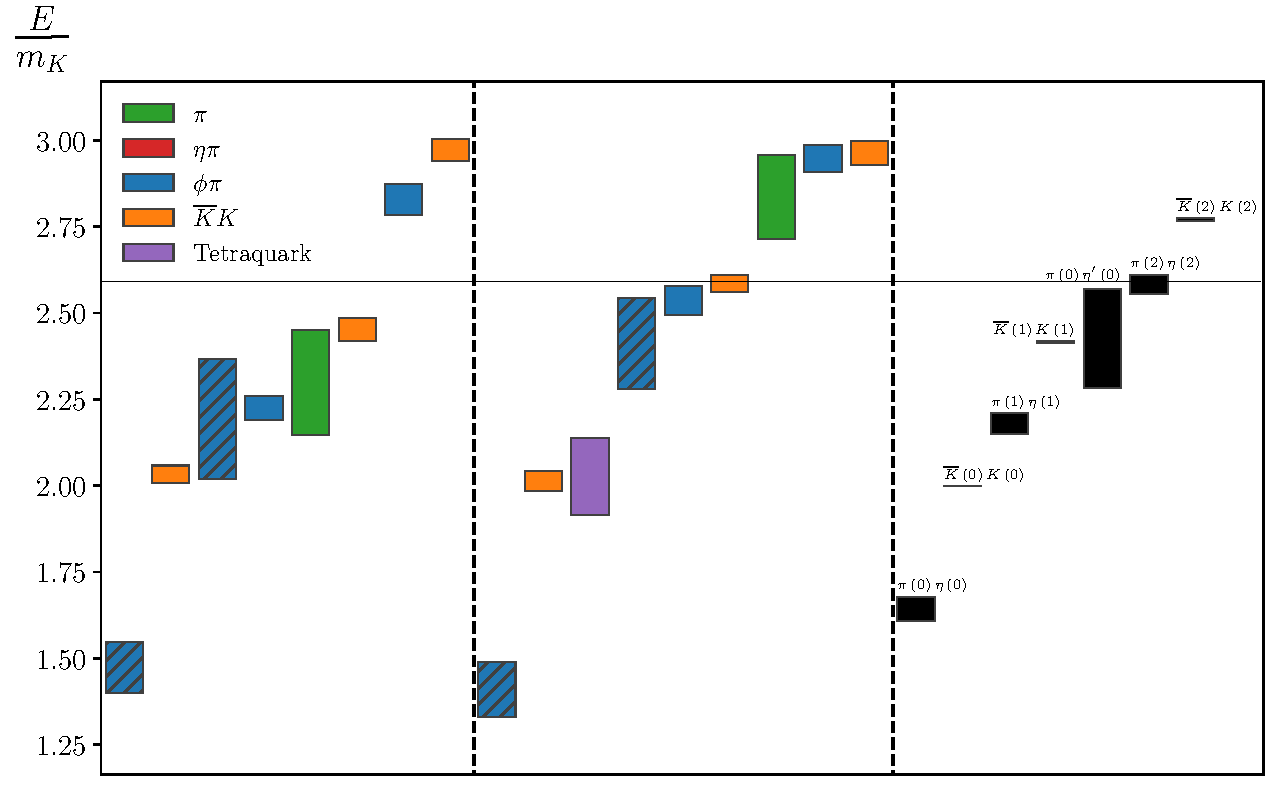
\includegraphics[width=1.5\textwidth]{figures/spectrum_a1gm/staircase.pdf}
  \caption{On the left: a spectrum obtained in the $a_0(980)$ channel using the operator basis given in Table~\ref{table:a0_ops_no_tq}, which contains no tetraquark operators. On the right: a spectrum obtained in the $a_0(980)$ channel using the same basis but with the addition of one tetraquark operator.}
  \label{fig:a0_spectrum}
\end{figure}

\begin{figure}
  \raisebox{-0.01in}{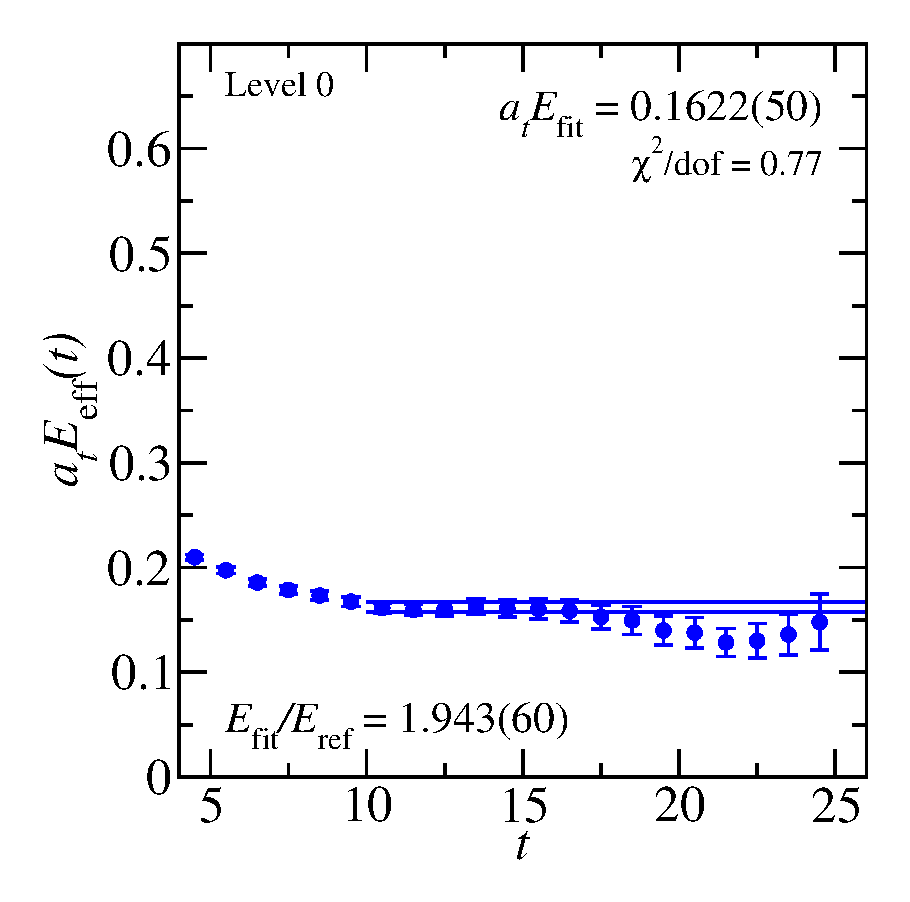
\includegraphics[width=0.325\textwidth]{figures/spectrum_a1gm/no_tq/fits/fit_0.pdf}}
  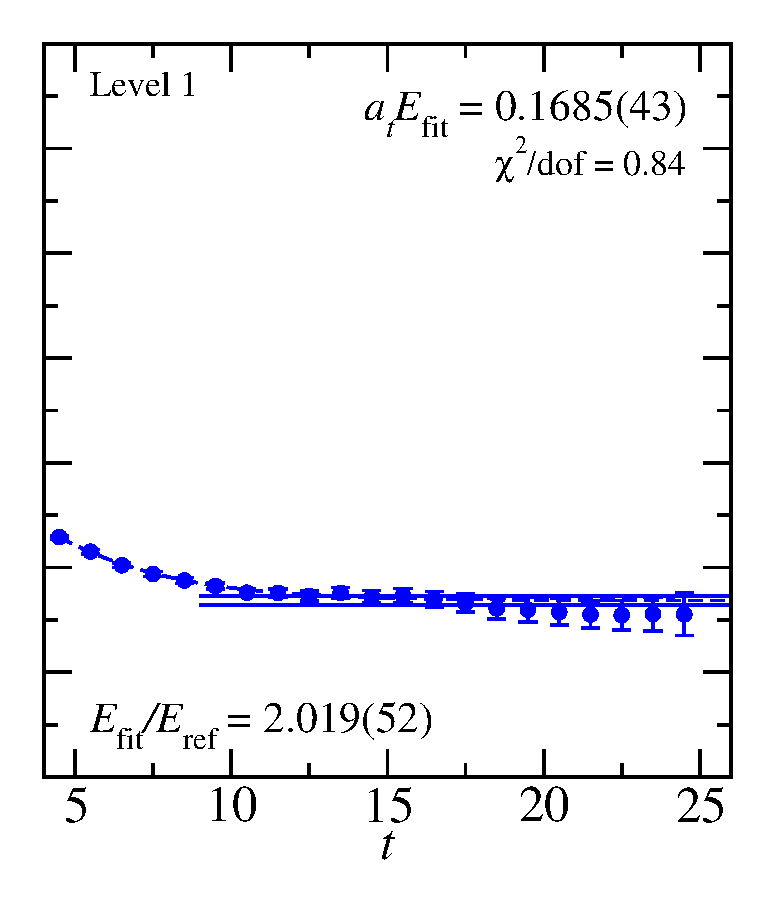
\includegraphics[width=0.28\textwidth]{figures/spectrum_a1gm/no_tq/fits/fit_1.pdf}
  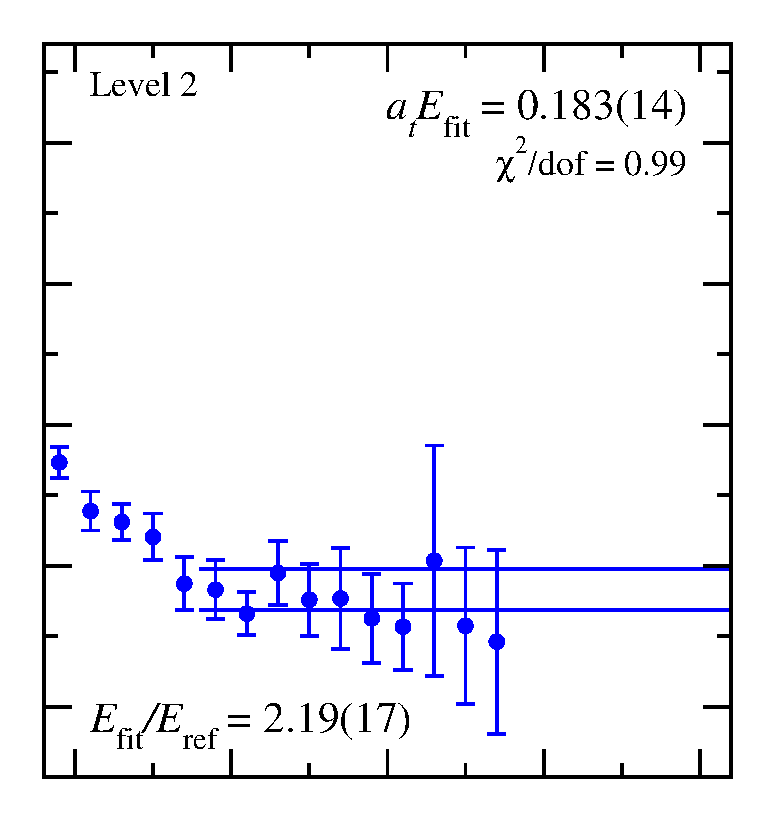
\includegraphics[width=0.28\textwidth]{figures/spectrum_a1gm/no_tq/fits/fit_2.pdf}\\
  \raisebox{-0.01in}{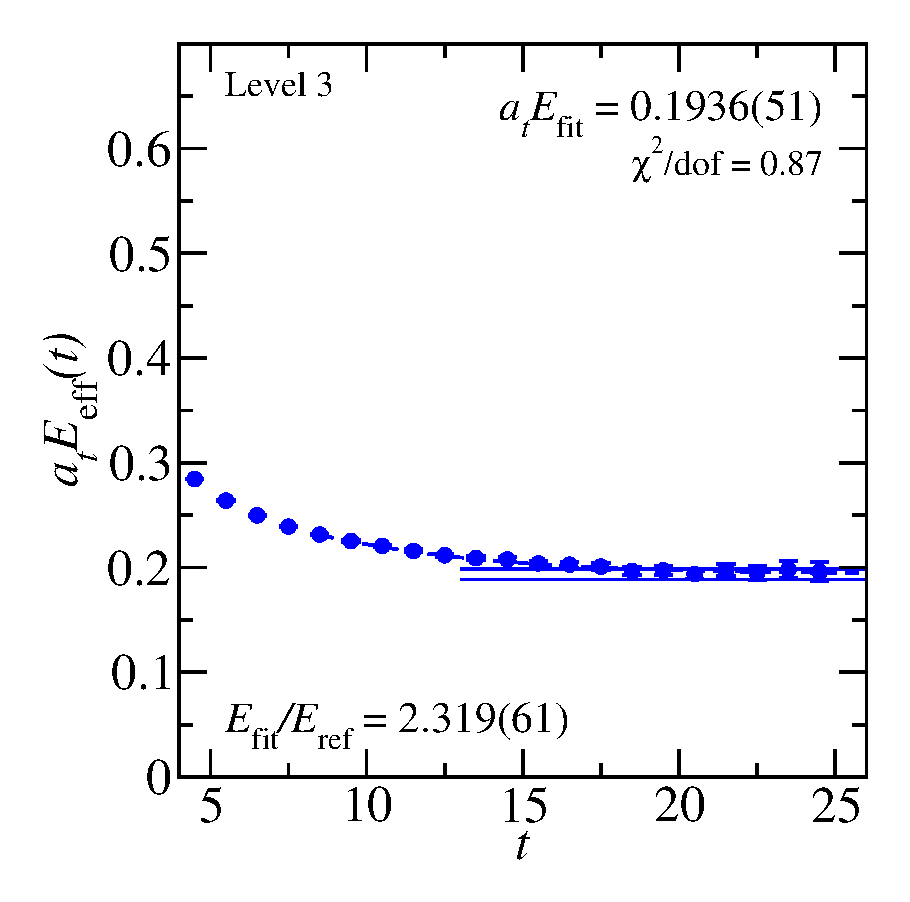
\includegraphics[width=0.325\textwidth]{figures/spectrum_a1gm/no_tq/fits/fit_3.pdf}}
  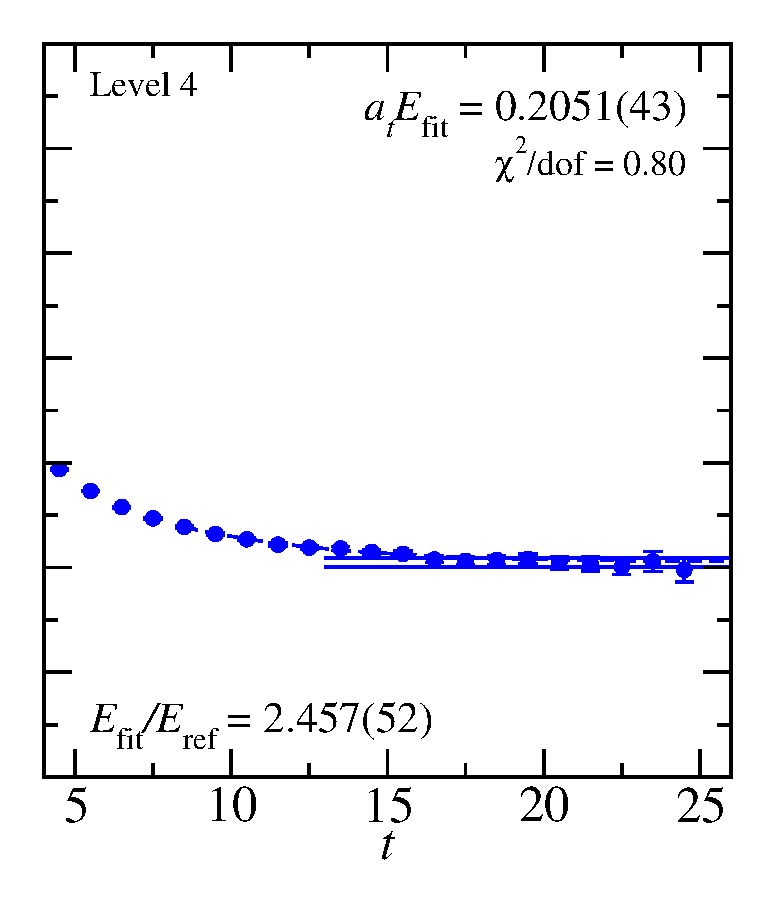
\includegraphics[width=0.28\textwidth]{figures/spectrum_a1gm/no_tq/fits/fit_4.pdf}
  \includegraphics[width=0.28\textwidth]{figures/spectrum_a1gm/no_tq/fits/fit_5.pdf}\\
  \raisebox{-0.01in}{\includegraphics[width=0.325\textwidth]{figures/spectrum_a1gm/no_tq/fits/fit_7.pdf}}
  \includegraphics[width=0.28\textwidth]{figures/spectrum_a1gm/no_tq/fits/fit_8.pdf}
  \includegraphics[width=0.28\textwidth]{figures/spectrum_a1gm/no_tq/fits/fit_6.pdf}\\
  \raisebox{-0.01in}{\includegraphics[width=0.325\textwidth]{figures/spectrum_a1gm/no_tq/fits/fit_9.pdf}}
  \includegraphics[width=0.28\textwidth]{figures/spectrum_a1gm/no_tq/fits/fit_10.pdf}
  \includegraphics[width=0.28\textwidth]{figures/spectrum_a1gm/no_tq/fits/fit_11.pdf}
  \caption{Effective energies for the rotated $12\times 12$ correlator matrix in the $a_0(980)$ channel, using an operator basis containing no tetraquark operators. Effective energy curves calculated from correlator fits are overlaid, and fit results are shown.}
  \label{fig:a0_no_tq_grid}
\end{figure}

\begin{figure}
  \includegraphics[width=0.3\textwidth]{figures/spectrum_a1gm/no_tq/zfactors/zfactor_pion-P000-A1gm_1-SS_0.pdf}
  \includegraphics[width=0.28\textwidth]{figures/spectrum_a1gm/no_tq/zfactors/zfactor_pion-P000-A1gm_1-SD_2.pdf}
  \includegraphics[width=0.28\textwidth]{figures/spectrum_a1gm/no_tq/zfactors/zfactor_pion-P000-A1gm_1-TDO_3.pdf}\\
  \includegraphics[width=0.3\textwidth]{figures/spectrum_a1gm/no_tq/zfactors/zfactor_isotriplet_phi_pion-A1gm_1-P000-A1up-SS_0-P000-A1um-SS_0.pdf}
  \includegraphics[width=0.28\textwidth]{figures/spectrum_a1gm/no_tq/zfactors/zfactor_isotriplet_kaon_kbar-A1gm_1-P000-A1u-SS_0-P000-A1u-SS_0.pdf}
  \includegraphics[width=0.28\textwidth]{figures/spectrum_a1gm/no_tq/zfactors/zfactor_isotriplet_phi_pion-A1gm_1-P001-A2p-SS_1-P00-1-A2m-SS_1.pdf}\\
  \includegraphics[width=0.3\textwidth]{figures/spectrum_a1gm/no_tq/zfactors/zfactor_isotriplet_kaon_kbar-A1gm_1-P001-A2-SS_1-P00-1-A2-SS_1.pdf}
  \includegraphics[width=0.28\textwidth]{figures/spectrum_a1gm/no_tq/zfactors/zfactor_isotriplet_phi_pion-A1gm_1-P011-A2p-SS_0-P0-1-1-A2m-SS_0.pdf}
  \includegraphics[width=0.28\textwidth]{figures/spectrum_a1gm/no_tq/zfactors/zfactor_isotriplet_phi_pion-A1gm_1-P000-T1um-SS_0-P000-T1up-SS_0.pdf}\\
  \includegraphics[width=0.3\textwidth]{figures/spectrum_a1gm/no_tq/zfactors/zfactor_isotriplet_eta_pion-A1gm_1-P000-T1um-SS_0-P000-T1up-SS_0.pdf}
  \includegraphics[width=0.28\textwidth]{figures/spectrum_a1gm/no_tq/zfactors/zfactor_isotriplet_eta_pion-A1gm_1-P001-A2p-SS_0-P00-1-A2m-SS_0.pdf}
  \includegraphics[width=0.28\textwidth]{figures/spectrum_a1gm/no_tq/zfactors/zfactor_isotriplet_eta_pion-A1gm_1-P011-A2p-SS_1-P0-1-1-A2m-SS_1.pdf}
  \caption{Overlap factors for the rotated $12\times 12$ correlator matrix in the $a_0(980)$ channel, using an operator basis containing no tetraquark operators.}
  \label{fig:a0_no_tq_zfactors}
\end{figure}

\begin{table}
  \centering
  \begin{tabular}{c|c|c|c|c}
    $E / E_K$ & $a_t E$ & Fit model & $(t_{\mathrm{min}}, {t_\mathrm{max}})$ & $\chi^2 / \rm{d.o.f.}$\\
    \hline
    1.943(60)&0.1622(50)&1{-}exp&$(10, 26)$&0.77\\
    2.019(52)&0.1685(43)&2{-}exp&$(3, 26)$&0.84\\
    2.020(56)&0.1687(47)&2{-}exp&$(9, 26)$&0.82\\
    2.319(61)&0.1936(51)&2{-}exp&$(7, 26)$&0.87\\
    2.457(52)&0.2051(43)&2{-}exp&$(7, 26)$&0.8\\
    2.759(41)&0.2303(34)&2{-}exp&$(7, 26)$&1.43\\
    2.88(66)&0.241(55)&1{-}exp&$(8, 15)$&0.29\\
    3.882(75)&0.3241(62)&2{-}exp&$(4, 26)$&1.39\\
    3.905(64)&0.3260(53)&1{-}exp&$(8, 23)$&0.7\\
    4.66(42)&0.389(35)&1{-}exp&$(8, 16)$&0.27\\
    6.23(16)&0.520(14)&1{-}exp&$(4, 15)$&0.58\\
    6.69(41)&0.559(34)&1{-}exp&$(4, 15)$&1.22
  \end{tabular}
  \caption{Fit details for the spectrum obtained in the $a_0(980)$ channel using the operator basis given in Table~\ref{table:a0_ops_no_tq}, which contains no tetraquark operators.}
  \label{table:a0_no_tq_spectrum}
\end{table}

\begin{figure}
  \raisebox{-0.01in}{\includegraphics[width=0.255\textwidth]{figures/spectrum_a1gm/with_tq/fits/fit_0.pdf}}
  \includegraphics[width=0.22\textwidth]{figures/spectrum_a1gm/with_tq/fits/fit_1.pdf}
  \includegraphics[width=0.22\textwidth]{figures/spectrum_a1gm/with_tq/fits/fit_3.pdf}
  \includegraphics[width=0.22\textwidth]{figures/spectrum_a1gm/with_tq/fits/fit_2.pdf}\\
  \includegraphics[width=0.255\textwidth]{figures/spectrum_a1gm/with_tq/fits/fit_4.pdf}
  \includegraphics[width=0.22\textwidth]{figures/spectrum_a1gm/with_tq/fits/fit_5.pdf}
  \includegraphics[width=0.22\textwidth]{figures/spectrum_a1gm/with_tq/fits/fit_6.pdf}
  \includegraphics[width=0.22\textwidth]{figures/spectrum_a1gm/with_tq/fits/fit_8.pdf}\\
  \raisebox{0.15in}{\includegraphics[width=0.255\textwidth]{figures/spectrum_a1gm/with_tq/fits/fit_7.pdf}}
  \includegraphics[width=0.22\textwidth]{figures/spectrum_a1gm/with_tq/fits/fit_9.pdf}
  \includegraphics[width=0.22\textwidth]{figures/spectrum_a1gm/with_tq/fits/fit_10.pdf}
  \includegraphics[width=0.22\textwidth]{figures/spectrum_a1gm/with_tq/fits/fit_11.pdf}\\
  \raisebox{0.1in}{\includegraphics[width=0.255\textwidth]{figures/spectrum_a1gm/with_tq/fits/fit_12.pdf}}
  \caption{Effective energies for the rotated $13\times 13$ correlator matrix in the $a_0(980)$ channel, using the same operator basis but with the addition of one tetraquark operator. Effective energy curves calculated from correlator fits are overlaid, and fit results are shown.}
  \label{fig:a0_with_tq_grid}
\end{figure}

\begin{figure}
  \includegraphics[width=0.24\textwidth]{figures/spectrum_a1gm/with_tq/zfactors/zfactor_pion-P000-A1gm_1-SS_0.pdf}
  \includegraphics[width=0.22\textwidth]{figures/spectrum_a1gm/with_tq/zfactors/zfactor_pion-P000-A1gm_1-SD_2.pdf}
  \includegraphics[width=0.22\textwidth]{figures/spectrum_a1gm/with_tq/zfactors/zfactor_pion-P000-A1gm_1-TDO_3.pdf}
  \includegraphics[width=0.22\textwidth]{figures/spectrum_a1gm/with_tq/zfactors/zfactor_tquudu3p-P000-A1gm_1-SS_2.pdf}\\
  \includegraphics[width=0.24\textwidth]{figures/spectrum_a1gm/with_tq/zfactors/zfactor_isotriplet_phi_pion-A1gm_1-P000-A1up-SS_0-P000-A1um-SS_0.pdf}
  \includegraphics[width=0.22\textwidth]{figures/spectrum_a1gm/with_tq/zfactors/zfactor_isotriplet_kaon_kbar-A1gm_1-P000-A1u-SS_0-P000-A1u-SS_0.pdf}
  \includegraphics[width=0.22\textwidth]{figures/spectrum_a1gm/with_tq/zfactors/zfactor_isotriplet_phi_pion-A1gm_1-P001-A2p-SS_1-P00-1-A2m-SS_1.pdf}
  \includegraphics[width=0.22\textwidth]{figures/spectrum_a1gm/with_tq/zfactors/zfactor_isotriplet_kaon_kbar-A1gm_1-P001-A2-SS_1-P00-1-A2-SS_1.pdf}\\
  \raisebox{0.12in}{\includegraphics[width=0.24\textwidth]{figures/spectrum_a1gm/with_tq/zfactors/zfactor_isotriplet_phi_pion-A1gm_1-P011-A2p-SS_0-P0-1-1-A2m-SS_0.pdf}}
  \includegraphics[width=0.22\textwidth]{figures/spectrum_a1gm/with_tq/zfactors/zfactor_isotriplet_phi_pion-A1gm_1-P000-T1um-SS_0-P000-T1up-SS_0.pdf}
  \includegraphics[width=0.22\textwidth]{figures/spectrum_a1gm/with_tq/zfactors/zfactor_isotriplet_eta_pion-A1gm_1-P000-T1um-SS_0-P000-T1up-SS_0.pdf}
  \includegraphics[width=0.22\textwidth]{figures/spectrum_a1gm/with_tq/zfactors/zfactor_isotriplet_eta_pion-A1gm_1-P001-A2p-SS_0-P00-1-A2m-SS_0.pdf}\\
  \raisebox{0.12in}{\includegraphics[width=0.24\textwidth]{figures/spectrum_a1gm/with_tq/zfactors/zfactor_isotriplet_eta_pion-A1gm_1-P011-A2p-SS_1-P0-1-1-A2m-SS_1.pdf}}
  \caption{Overlap factors for the rotated $13\times 13$ correlator matrix in the $a_0(980)$ channel, using the same operator basis given in Table~\ref{table:a0_ops_no_tq}, with the addition of one tetraquark operator.}
  \label{fig:a0_with_tq_zfactors}
\end{figure}

\begin{table}
  \centering
  \begin{tabular}{c|c|c|c|c}
    $E / E_K$ & $a_t E$ & Fit model & $(t_{\mathrm{min}}, {t_\mathrm{max}})$ & $\chi^2 / \rm{d.o.f.}$\\
    \hline
    1.939(59)&0.1619(49)&1{-}exp&$(10, 26)$&0.74\\
    2.019(52)&0.1685(43)&2{-}exp&$(3, 26)$&0.82\\
    2.038(56)&0.1702(46)&2{-}exp&$(8, 26)$&1.18\\
    2.27(15)&0.189(13)&1{-}exp&$(10, 20)$&1.33\\
    2.318(60)&0.1935(50)&2{-}exp&$(7, 26)$&0.76\\
    2.455(52)&0.2049(43)&2{-}exp&$(7, 26)$&0.72\\
    2.767(41)&0.2310(34)&2{-}exp&$(7, 26)$&1.48\\
    2.90(63)&0.242(52)&1{-}exp&$(8, 15)$&0.28\\
    3.837(97)&0.3203(81)&1{-}exp&$(9, 22)$&0.78\\
    3.914(70)&0.3268(58)&2{-}exp&$(3, 26)$&1.26\\
    4.64(42)&0.387(35)&1{-}exp&$(8, 16)$&0.27\\
    6.23(16)&0.520(13)&1{-}exp&$(4, 15)$&0.55\\
    6.69(41)&0.559(34)&1{-}exp&$(4, 15)$&1.27
  \end{tabular}
  \caption{Fit details for the spectrum obtained in the $a_0(980)$ channel using the operator basis given in Table~\ref{table:a0_ops_no_tq}, with the addition of one tetraquark operator.}
  \label{table:a0_with_tq_spectrum}
\end{table}